%! Author = matteomagnini
%! Date = 05/03/25

%----------------------------------------------------------------------------------------
\chapter{Autonomous learning systems}
\label{ch:autonomous-learning-systems}
\minitoc
%----------------------------------------------------------------------------------------


This is arguably the most important chapter of the thesis, the crucial moment when all the bricks come together.
%
Here we present key contributions of the PhD towards the development of autonomous learning systems exploiting \gls{SKI} and \gls{SKE}.
%
In particular, we make use of \gls{SKE} to systematically extract symbolic knowledge from a trained sub-symbolic model, and conversely, we exploit \gls{SKI} to provide the sub-symbolic model with relevant context information.
%
This cycle between \gls{SKI} and \gls{SKE} is an early idea of my PhD, and it is presented in~\Cref{sec:cycle-ski-ske}.


\note{Add references for this section}
%
The goal of autonomous learning systems is straightforward: to create systems that can learn -- and possibly adapt -- independently, without requiring constant human intervention.
%
The knowledge that is learnt can be presented in many forms.
%
We discussed in details about the differences between symbolic and sub-symbolic representations in~\Cref{ch:ai} and also the many forms of symbolic knowledge that can be used to represent knowledge, such as rules, ontologies, and knowledge graphs~\Cref{sec:symbolic-ai}.
%
We believe that the knowledge learnt by autonomous learning systems should be represented symbolically.
%
The advantages of symbolic representations are many, as we discussed in~\Cref{sec:symbolic-ai}.
%
Here, we recall the most important ones:
%
\begin{inlinelist}
    %
    \item interpretability: symbolic knowledge is human-readable, which makes it easier to understand and verify;
    %
    \item reasoning: symbolic knowledge can be used to perform logical reasoning;
    %
    \item transferability: symbolic knowledge can be easily transferred between different systems and domains, which makes it more versatile;
    %
    \item model compression: symbolic knowledge can be more compact than sub-symbolic representations, which makes it more efficient;
    %
    \item model checking: symbolic knowledge can be formally verified, which makes it more reliable.
    %
\end{inlinelist}


On the other hand, sub-symbolic models have recently reached impressive performance in many tasks, especially in \gls{NLP} and \gls{NLG}, thanks to the advent of \glspl{LLM}.
%
Indeed, \glspl{LLM} are de-facto the new drivers of \gls{AI}.
%
Their presence is already ubiquitous, and they are used daily by millions of people.
%
Many \glspl{LLM} are so good at understanding and generating natural language that they can be considered as domain experts in many fields.
%
Still, limitations exist, and the possibility to generate hallucinations is always present.


In the following sections, we will present first the conceptual \gls{SKI}-\gls{SKE} loop, and then two main contributions towards the development of autonomous learning systems.
%
Both contributions exploit \glspl{LLM} to generate or finetune symbolic knowledge about specific domains.


\section{Bridging Symbolic and Sub-symbolic \gls{AI}}
\label{sec:cycle-ski-ske}
%
In the discussion paper ``Bridging Symbolic and Sub-symbolic AI: Towards Cooperative Transfer Learning in Multi-Agent Systems''~\cite{DBLP:conf/aiia/MagniniCO22} presented at the 22nd International Conference of the Italian Association for Artificial Intelligence (AIxIA 2022), we introduced the ideas of a loop between \gls{SKI} and \gls{SKE} processes in the context of \glspl{MAS}.
%
For computational agents, algorithms exist to mimic basic cognitive capabilities such as induction, communication, knowledge representation, and reasoning.
%
These capabilities are developed under the domains of symbolic \gls{AI} and \gls{ML}.
%
However, unlike humans, symbolic \gls{AI} and \gls{ML} algorithms are typically designed to solve specific tasks and do not inherently support interaction, cooperation, or knowledge exchange.


This work proposes that \gls{ML}-based intelligent systems can benefit from symbolic knowledge exchange to enhance their learning capabilities~\cite{imagination-extraamas2021,not-just-for-humans-omicini-2020,expectation-extraamas2021}.
%
We argue that symbolic knowledge exchange can play a crucial role in enabling software agents to achieve the ability to \emph{learn to learn} new tasks.


We introduce two types of intelligent systems: \gls{CoL} and \gls{CoTL}.
%
\Gls{CoL} systems are \glspl{MAS} in which agents can retrieve or provide knowledge about specific tasks to or from other agents.
%
This knowledge can be used during learning or inference.
%
\gls{CoTL} systems extend \gls{CoL} systems by enabling agents to acquire, exploit, and combine knowledge about related tasks to learn novel tasks they were not explicitly designed for.
%
Both systems aim to mimic the learning processes of human societies, albeit to varying extents.
%
Agents in these systems collaborate by sharing symbolic and, potentially, sub-symbolic knowledge about their tasks, similar to human interactions.

This chapter outlines a roadmap for leveraging knowledge representation and sharing to achieve higher levels of artificial intelligence through \gls{CoL} and \gls{CoTL} systems.
%
We analyze the requirements of these systems in relation to the state of the art and discuss their potential implementation.
%

\subsection{Background}
\label{subsec:background}

\subsubsection{Symbolic and Sub-symbolic}
\label{subsubsec:symbolic-and-sub-symbolic}
%
Symbolic and sub-symbolic representations are two fundamental paradigms for knowledge representation, extensively discussed in~\Cref{ch:ai,sec:symbolic-ai}.
%
Symbolic representations, such as propositional logic, \glspl{KG}, and \gls{FOL}, are interpretable, compact, and versatile, supporting both intensional and extensional knowledge representation~\cite{DBLP:conf/ogai/Gelder90,DBLP:conf/aiia/CiattoCOC19}.
%
These properties make them suitable for tasks requiring reasoning, transferability, and formal verification.
%
In contrast, sub-symbolic representations, commonly used in \gls{ML} and \glspl{NN}, encode knowledge as numerical arrays and functions, often treated as black-box models due to their complexity~\cite{interpretability-lipton-2018}.
%
Despite their lack of interpretability, they excel in performance across various tasks.
%
The interplay between these paradigms is explored through \gls{SKE} and \gls{SKI}, as introduced in~\Cref{sec:ske,sec:ski}.
%
\gls{SKE} extracts symbolic knowledge from sub-symbolic models, aiding interpretability and training, while \gls{SKI} injects symbolic knowledge into sub-symbolic models to enhance their efficiency and accuracy~\cite{survey-ske-andrews-1995,survey-ski-besold-2017}.
%

\subsubsection{Transfer vs.\ Multi-Task Learning}
\label{subsubsec:tl-mtl}
%
A \emph{task} in \gls{ML} refers to any supervised learning problem.
%
\Gls{TL} enables a predictor \(P\) trained on a task \(T'\) to transfer knowledge \(K\) to another predictor \(P'\) targeting a related task \(T\).
%
The primary goals of \gls{TL} are to:
%
\begin{inlinelist}
    \item reduce the data required to train \(P'\),
    %
    \item accelerate training, and
    %
    \item improve predictive performance.
    %
\end{inlinelist}

\Gls{TL} methods vary in \emph{what}, \emph{how}, and \emph{when} to transfer knowledge~\cite{survey-transfer-learning-sinno-2010}.
%
Most \gls{TL} techniques focus on sub-symbolic knowledge transfer, such as reusing shallow layers of a \gls{NN}~\cite{cnn-tl-imagenet-shin-2016}.
%
To date, no \gls{TL} methods explicitly leverage symbolic knowledge transfer.

\gls{MTL} extends \gls{TL} by training multiple predictors \(P_1, \dots, P_m\) on a set of related tasks \(\{T_1, \dots, T_m\}\) simultaneously~\cite{multi-task-learning-caruana-1997}.
%
This approach allows each predictor to benefit from the knowledge shared across tasks~\cite{survey-multi-task-learning-zhang-2021}.
%
Unlike \gls{TL}, where knowledge flows in one direction, \gls{MTL} facilitates bidirectional knowledge transfer.

\gls{MTL} techniques are classified based on whether they target \emph{homogeneous} or \emph{heterogeneous} tasks~\cite{survey-heterogeneous-transfer-learning-day-2017}.
%
Homogeneous tasks share the same input and output attributes, differing only in data distribution.
%
Heterogeneous tasks, on the other hand, have distinct attributes with little or no overlap.

In \gls{MTL}, determining task similarity remains an open challenge, particularly for heterogeneous tasks.
%
Empirical methods, such as testing performance improvements with \gls{MTL}, are often used to assess task relatedness.


\subsection{Contributions}
\label{subsec:contributions}

\subsubsection{\gls{CoL}}
\label{subsubsec:col}
%
\begin{figure*}[t]
    \centering
    \begin{subfigure}[t]{0.49\linewidth} % <--- [t] per top alignment
        \centering
        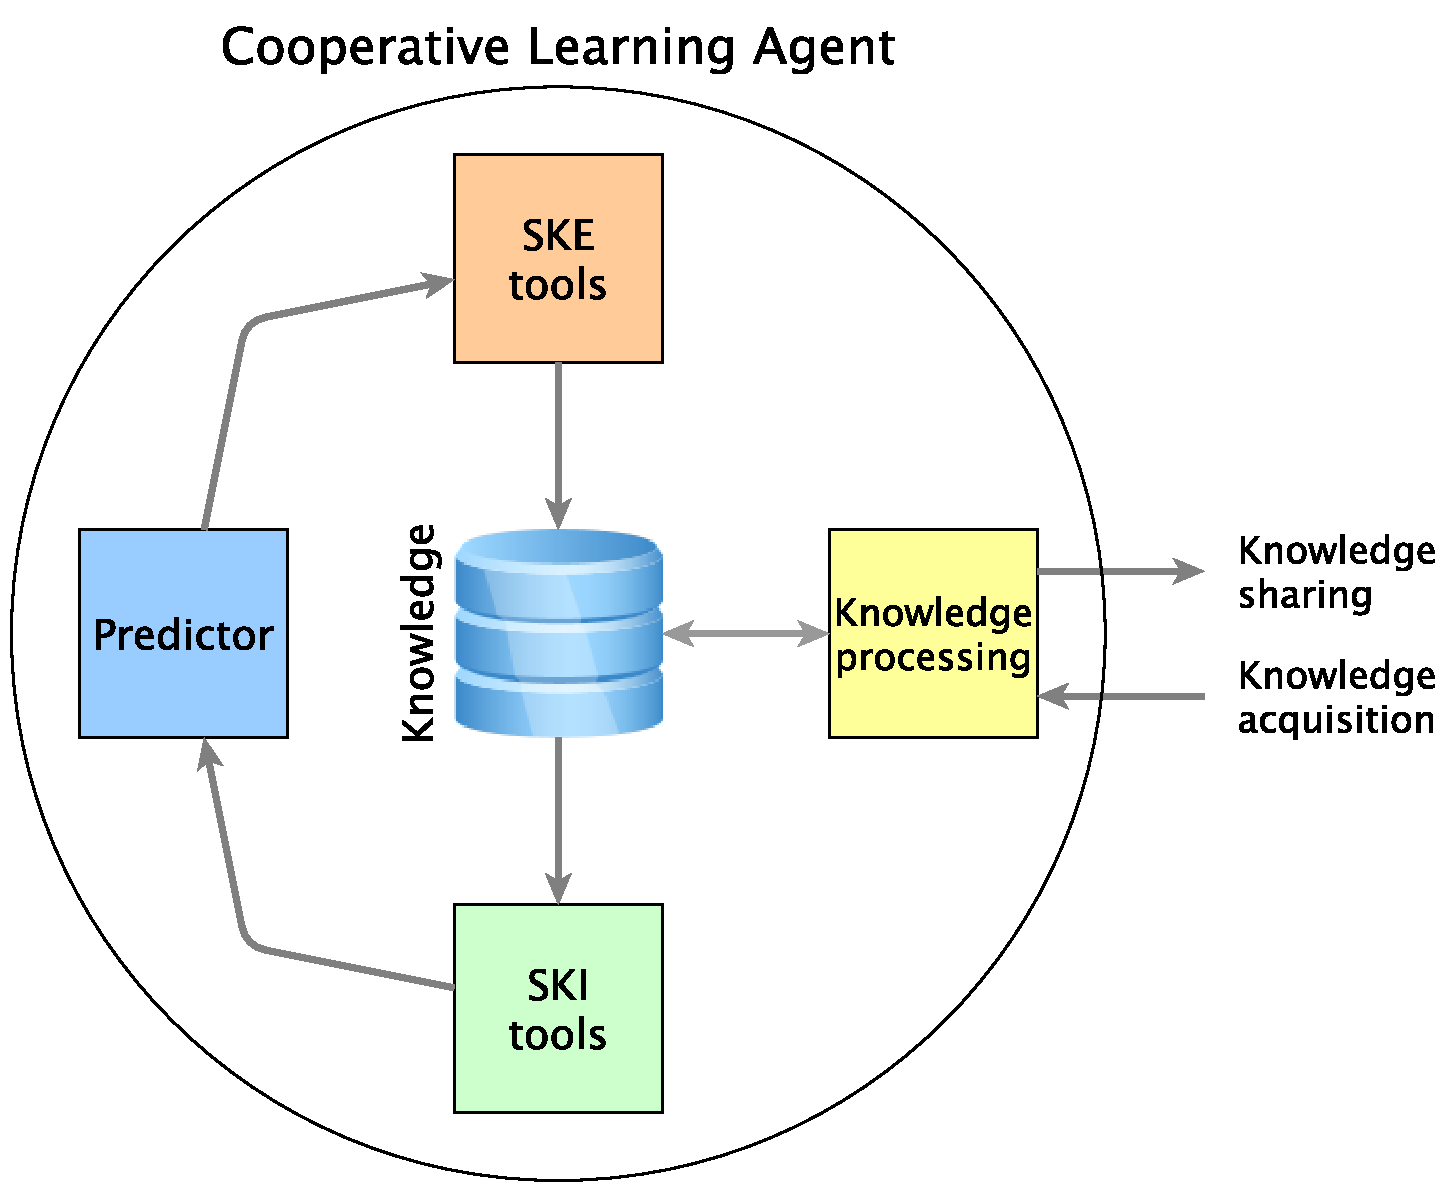
\includegraphics[width=\linewidth]{figures/cl-agent}
        \caption{
            Agent's architecture for \gls{CoL}.
            %
            The agent is equipped with a set of \gls{SKE} and \gls{SKI} methods to manipulate knowledge, plus some functions to pre/post-process knowledge.
        }
        \label{fig:cl-agent-architecture}
    \end{subfigure}%
    \hfill
    \begin{subfigure}[t]{0.49\linewidth} % <--- [t] per top alignment
        \centering
        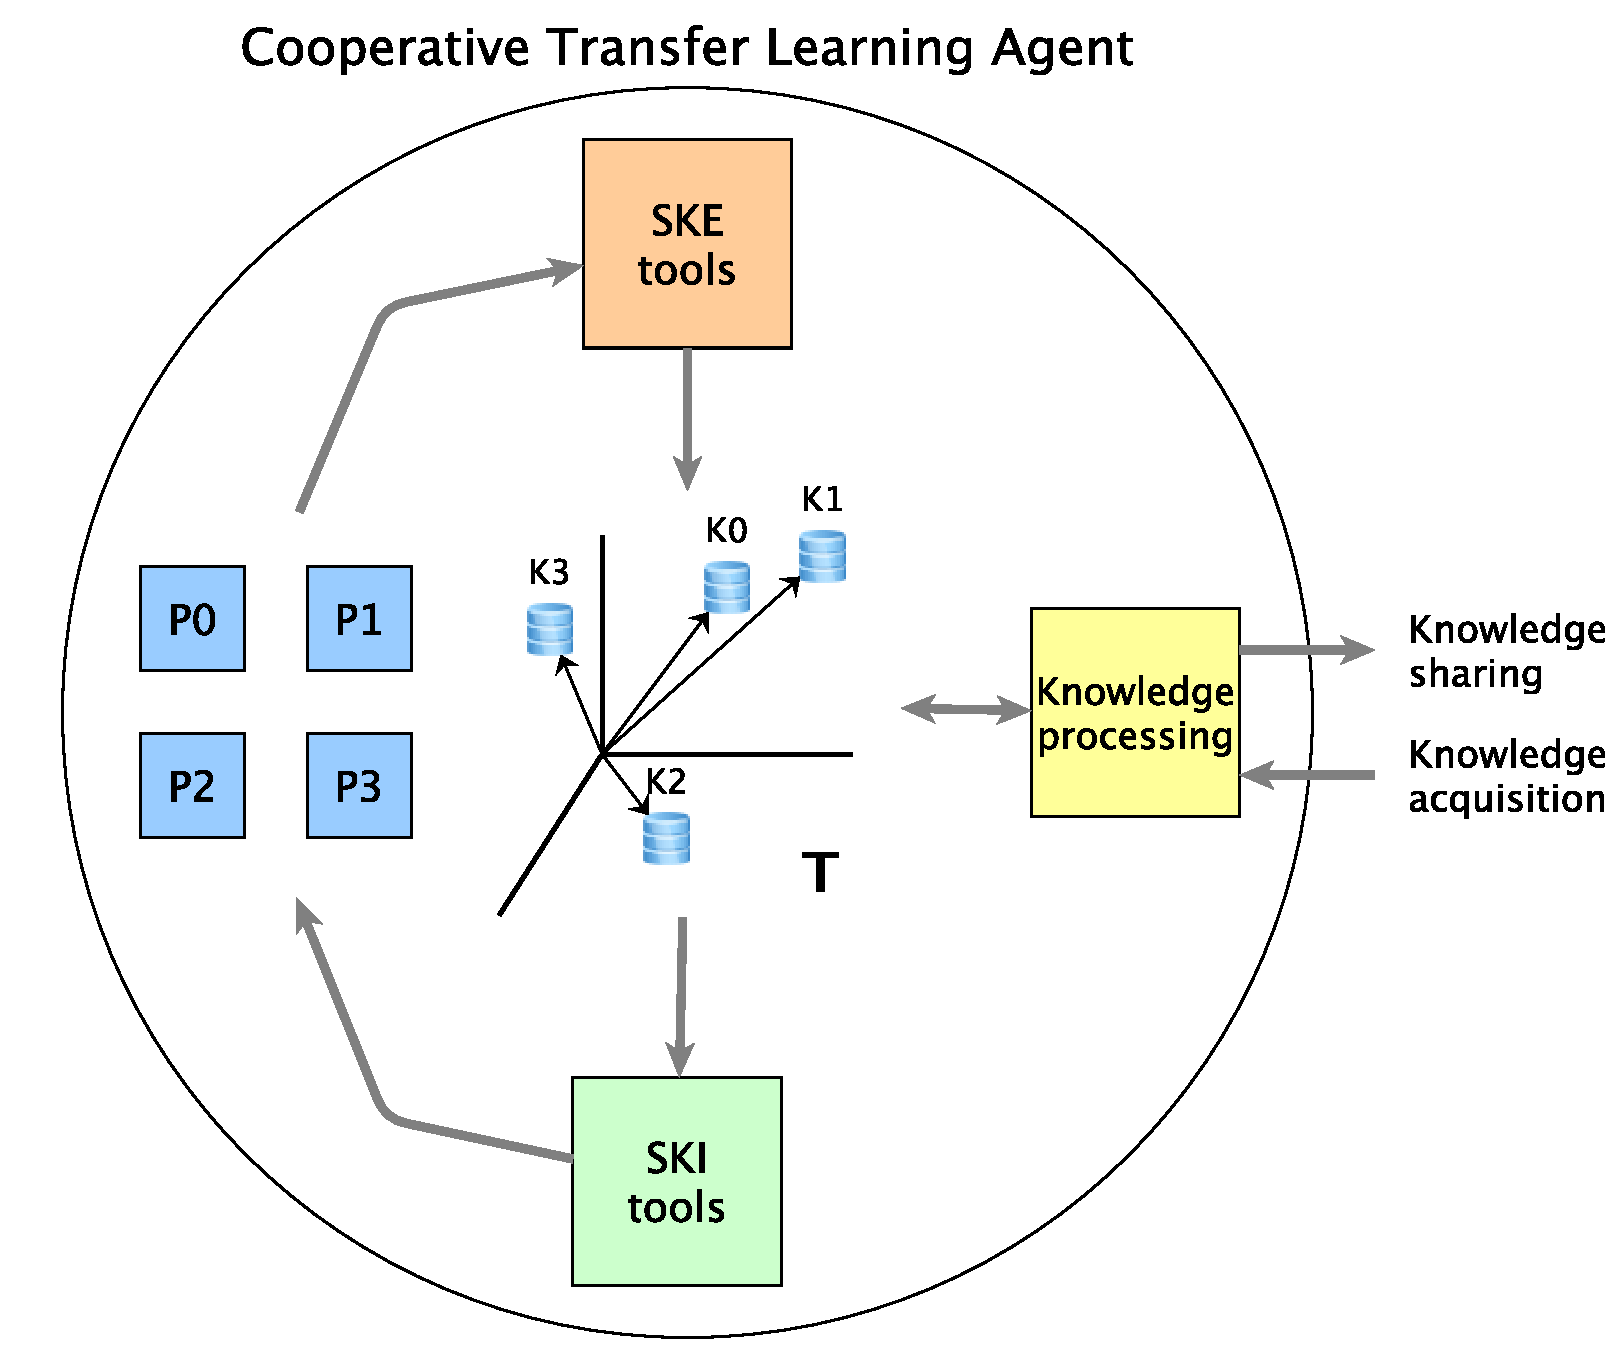
\includegraphics[width=\linewidth]{figures/ctl-agent}
        \caption{
            Agent's architecture for \gls{CoTL}.
            %
            The agent is equipped with a set of \gls{SKE} and \gls{SKI} methods to manipulate knowledge, functions to pre/post-process knowledge, plus a task space and relatedness functions to evaluate if two different tasks are related.
            %
            Each task in the task space $T$ is paired with its specific knowledge. For each task the agent has at least one predictor.
            %
            In the example are represented the knowledge of four tasks but they can come in arbitrary number.}
        \label{fig:ctl-agent-architecture}
    \end{subfigure}
    \caption{Architectures for \gls{CoL} and \gls{CoTL} agents.}
    \label{fig:architectures}
\end{figure*}

%
A \gls{CoL} system is a \gls{MAS} where agents can exchange knowledge about specific tasks.
%
This exchange includes both retrieving knowledge from other agents and providing knowledge when requested.
%
Symbolic knowledge sharing is particularly crucial, as it enables effective agent-to-agent communication and transfer~\cite{not-just-for-humans-omicini-2020}.
%
% Symbolic knowledge is preferred due to its interpretability and transferability.

To enable \gls{CoL}, agents must possess the following capabilities:
%
\begin{enumerate}
    \item\label{capability:learning} learning from experience and adapting their behavior accordingly,
    %
    \item\label{capability:extraction} representing their internal behavior in a symbolic format,
    %
    \item\label{capability:injection} updating their behavior based on symbolic specifications,
    %
    \item\label{capability:interaction} interacting with other agents to exchange symbolic knowledge.
\end{enumerate}
%
Capabilities~\ref{capability:extraction} and~\ref{capability:injection} are complementary.
%
When combined with~\ref{capability:interaction}, they facilitate cooperative learning through interaction.
%
Capability~\ref{capability:learning} ensures that agents can independently acquire new behaviors.

In practice, \gls{CoL} systems often rely on sub-symbolic \gls{ML} to support capability~\ref{capability:learning}.
%
Each agent is typically equipped with an \gls{ML} predictor to learn from local data.
%
Since \glspl{MAS} often consist of heterogeneous agents with diverse purposes, multiple types of predictors may coexist within the same system.

To support capability~\ref{capability:interaction}, agents must agree on a shared symbolic representation for describing and exchanging behavioral specifications.
%
\gls{SKE} and \gls{SKI} techniques are instrumental in enabling capabilities~\ref{capability:extraction} and~\ref{capability:injection}, respectively.

%
\Cref{fig:cl-agent-architecture} illustrates the architecture of a \gls{CoL} agent.
%
Each agent is equipped with one or more \gls{SKE} and \gls{SKI} algorithms to handle symbolic knowledge input and output.
%
When queried, an agent extracts symbolic knowledge from its internal \gls{ML} predictor using \gls{SKE} and shares it with the requesting agent.
%
The recipient agent can then update its predictor by injecting the received knowledge using \gls{SKI}.
%
Pre- and post-processing steps, such as pruning or merging formulas, may be applied to regulate the transferred knowledge.

Key design considerations for \gls{CoL} systems include:
%
\begin{inlinelist}
    \item\label{itm:logic-formalism} selecting appropriate formalisms for knowledge representation, and
    %
    \item\label{itm:arsenal} choosing suitable \gls{SKI}/\gls{SKE} techniques based on the predictors' knowledge representation.
\end{inlinelist}
%
For~\ref{itm:logic-formalism}, while \gls{FOL} offers high expressiveness, it may limit the availability of compatible techniques.
%
Less expressive logics, such as propositional logic, may also be considered for practical reasons.

Agents can be trained without prior knowledge.
%
During training, they can extract knowledge, combine it with knowledge from other agents, inject it back, and continue training.
%
This iterative process, known as the train-extract-fix-inject cycle, improves the agent's performance over time.
%
With each cycle, the extracted knowledge becomes increasingly accurate, as the predictor itself improves.


\subsubsection{\gls{CoTL}}
\label{subsubsec:cotl}
%
A \gls{CoTL} system extends \gls{CoL} by enabling agents to leverage knowledge from related tasks to learn \emph{novel} tasks.
%
The ultimate goal of \gls{CoTL} systems is to enable agents to ``learn to learn.''

The concept of learning to learn builds on the definition of \gls{ML}~\cite{DBLP:books/daglib/0087929} and was introduced in~\cite{learning-to-learn-thrun-1998}.
%
Formally, given:
%
\begin{itemize}
    \item a set of tasks \(\mathcal{T} = \{T_{1}, \dots, T_{n}\}\),
    %
    \item trainable experience for each task \(\mathcal{E} = \{E_{1}, \dots, E_{n}\}\), such as \gls{ML} predictors or symbolic knowledge bases, and
    %
    \item a performance measure \(f_i : \mathcal{T} \times \mathcal{E} \rightarrow \mathbb{R}\) for each task,
\end{itemize}
%
an agent is capable of learning to learn if \(f_i\) improves as a function of all items in \(\mathcal{E}\) and the number of tasks \(n\).

Practical aspects of \gls{CoTL} include determining \emph{when} and \emph{how} to transfer experience.
%
For the `when,' agents must autonomously compute task similarity, as manual intervention is infeasible.
%
Similarity measures, such as distance-based or learning-based methods, can be employed~\cite{multi-task-learning-caruana-1997}.

For the `how,' the approach depends on whether tasks are \emph{homogeneous} or \emph{heterogeneous}.
%
Homogeneous tasks share input and output spaces but differ in data distribution, allowing straightforward knowledge transfer.
%
Heterogeneous tasks, however, differ in both input and output features, requiring more complex strategies.

Consider two heterogeneous classification tasks \(T_1\) and \(T_2\) with knowledge bases \(K_1\) and \(K_2\) composed of Horn clauses.
%
Knowledge transfer can proceed as follows:
%
\begin{enumerate}
    \item\label{itm:overlap-rule} If a rule \(r \in K_1 \cup K_2\) refers only to shared input features and classes, it can be used as-is.
    %
    \item\label{itm:quasi-overlap-rule} If \(r\)'s body refers to shared features but its head targets task-specific classes, \gls{SKI} techniques or class mappings may be required.
    %
    \item If \(r\) involves both shared and task-specific features:
    %
    \begin{enumerate}
        \item Relax the rule to include only shared features, then apply step~\ref{itm:overlap-rule}.
        %
        \item Map task-specific features between tasks~\cite{survey-heterogeneous-transfer-learning-day-2017}, then apply step~\ref{itm:overlap-rule}.
        %
        \item If neither is possible, discard the rule.
    \end{enumerate}
\end{enumerate}
%
This procedure can be adapted for other tasks, such as regression, and other knowledge representations.

%
\Cref{fig:ctl-agent-architecture} depicts the architecture of a \gls{CoTL} agent.
%
In addition to \gls{SKE} and \gls{SKI} algorithms, \gls{CoTL} agents require a task similarity function \(\sigma : \mathcal{T}^2 \rightarrow \mathbb{R}_{\geq 0}\) to evaluate task relatedness.

Another design consideration is the criterion for selecting knowledge from related tasks.
%
For example, designers may use a threshold-based approach, selecting knowledge from tasks with a similarity score above a certain threshold.
%
Alternatively, the \(k\) most similar tasks can be chosen.


\subsection{Discussion and conclusions}
\label{subsec:discussion-conclusions}

The integration of symbolic and sub-symbolic knowledge representations, along with knowledge manipulation tools, represents a promising direction for advancing \glspl{MAS}.
%
This approach aims to mimic the knowledge-sharing capabilities of human societies.
%
It has the potential to address several limitations in the current state of the art.
%
For instance, \gls{TL} focuses exclusively on sub-symbolic knowledge, which lacks human interpretability.
%
Similarly, \gls{MTL} requires simultaneous training on related tasks, posing scalability challenges.
%
Moreover, \gls{MTL} is currently limited to sub-symbolic knowledge alone.
%

\gls{CoL} and \gls{CoTL} systems offer significant opportunities for the development of intelligent systems.
%
Some of their key advantages include:
%
\begin{inlinelist}
    \item providing more accurate and human-interpretable explanations for tasks;
    %
    \item improving the performance of agents or predictors in solving individual tasks;
    %
    \item enabling improvements in one agent to positively influence others;
    %
    \item facilitating knowledge transfer between tasks, leading to improvements across multiple domains;
    %
    \item supporting continuous and automated learning without human intervention.
\end{inlinelist}
%

Despite these advantages, several challenges remain.
%
First, while many \gls{SKE} and \gls{SKI} algorithms have been proposed, their practical implementations are still rare.
%
Second, determining task similarity in \gls{CoTL} systems is non-trivial and can significantly impact system performance.
%
Third, trust mechanisms must be considered.
%
For example, how reliable is the knowledge received by an agent?
%
What is the reputation of the knowledge source?
%
Finally, there is a need for datasets -- likely smaller than those required for systems without \gls{CoL} and \gls{CoTL} -- to train predictors effectively on new tasks.
%
Humans, for instance, can perform new tasks with minimal training, often relying solely on explanations (e.g., learning to play a new game).
%
Achieving such capabilities would mark a significant step toward artificial general intelligence.
%

In summary, this work introduces the novel concepts of \gls{CoL} and \gls{CoTL} within the scope of \glspl{MAS}.
%
These systems integrate symbolic and sub-symbolic knowledge representations and manipulation tools to emulate the learning processes of human societies.
%
We propose a general agent architecture for both \gls{CoL} and \gls{CoTL}, highlighting their advantages and limitations.
%





\section{\Glspl{LLM} as oracles for instantiating ontologies with domain-specific knowledge}
\label{sec:llm-as-oracles-for-instantiating-ontologies-with-domain-specific-knowledge}
%
In this section we present the paper ``Large language models as oracles for instantiating ontologies with domain-specific knowledge''~\cite{DBLP:journals/kbs/CiattoAMO25}, which is published in the international journal \emph{Knowledge-Based Systems}.

The demand for intelligent systems capable of understanding, reasoning, and interacting with complex information is rapidly increasing.
%
The development of such systems relies on the integration of machine-interpretable knowledge representations that can encapsulate human domain-specific knowledge across diverse fields.


The proliferation of data and its varied representation formats raises the question: \emph{How can domain-specific information be precisely represented in a machine-understandable manner?}
%
The answer lies in the concept of ontology~\cite{DBLP:books/daglib/p/Grimm10}.
%
Ontologies are formal, extensional representations of knowledge based on the principles of \glspl{DL}.
%
They define concepts, relationships, and properties in a structured, machine-readable format, enabling computational systems to reason about the world in a manner akin to human cognition.


Unlike sub-symbolic approaches, which rely on distributed or loosely organized data~\cite{DBLP:journals/csur/CiattoSAMO24}, ontologies provide a structured framework.
%
This framework bridges the \emph{semantic gap}, allowing \gls{AI} systems to move beyond superficial pattern recognition and grasp the underlying meaning of data.
%
From a human perspective, ontologies offer a shared vocabulary and an unambiguous understanding of domain-specific knowledge.
%
However, creating ontologies is a meticulous and time-consuming process, requiring adherence to the real-world domain they represent.


Currently, ontology population is performed either manually by domain experts or communities, or through semi-automatic extraction from data~\cite{petasis-2011}.
%
Manual population, while time-intensive and prone to human error, can yield high-quality results if the process is thorough and inclusive.
%
In contrast, data-driven approaches offer speed and scalability but may result in lower-quality ontologies due to biases in the data or limitations in the extraction process.


An ideal ontology population method would combine human- and data-driven approaches.
%
The former would refine and validate the ontology, while the latter would provide the necessary volume of instances.
%
To this end, we introduce \llmfkg, a novel approach that amalgamates the strengths of both methods.


Leveraging the observation that \glspl{LLM} are trained on diverse data from the web, we hypothesize that these models encapsulate substantial domain-specific knowledge.
%
\llmfkg{} is an automated procedure designed to extract this knowledge from \glspl{LLM} and use it to populate ontologies.
%
Starting with an initial schema of interrelated classes and properties, and a set of query templates, the method queries the \gls{LLM} multiple times.
%
It generates instances for classes, relationships, and properties based on the responses.
%
Further queries refine the ontology and balance the class hierarchy, ensuring compliance with the initial schema.
%
The result is an enriched ontology that experts can review, adjust, or complement as needed.


Our method has several advantages over state-of-the-art approaches.
%
First, it is not tied to any specific dataset, as it uses \glspl{LLM} as oracles to generate data.
%
Second, it supports both ontology population and refinement, making it incremental and applicable to pre-existing ontologies.
%
Finally, it is general-purpose, suitable for various domains and different \glspl{LLM}.


To validate our approach, we implemented \llmfkg{} in Python and used it to populate a custom \gls{OWL} ontology.
%
We evaluated the quality of the populated ontology through a detailed inspection of the generated instances, assessing their meaningfulness and placement within the ontology structure.
%
The experiment was repeated with different \glspl{LLM}, and the results were compared.


In summary, our method contributes to the ongoing discourse on ontology population by presenting a hybrid approach that leverages the capabilities of \glspl{LLM}.
%
To further analyze the strengths, weaknesses, opportunities, and threats of our approach, we dedicate a section to a detailed \gls{SWOT} analysis.


\subsection{Related work}
\label{subsec:related-work-kgfiller}

\paragraph{Ontology Population}
\label{par:related-workd-ontology-population}
%
The task of populating ontologies with instances, commonly referred to as \emph{ontology population}, is well-established in the semantic web community~\cite{lubani-2019}.
%
This process involves expanding an ontology with additional assertions, also known as \emph{ABox axioms}, while ensuring compliance with the concepts and properties defined in the \emph{TBox axioms}.
%
Some authors use the term \emph{ontology learning} to emphasize the (semi-)automatic inference of the entire ontology, including TBox axioms.
%
However, in this work, we adhere to the term \emph{ontology population}.


The need for (semi-)automatic ontology population arises from the limitations of manual methods, which are time-consuming, error-prone, and inherently costly~\cite{cherifa-2021}.
%
To address these challenges, various methods for structured data extraction from text have been proposed.
%
These methods can be broadly categorized into \emph{linguistics-based} and \gls{ML} approaches.


Linguistics-based approaches~\cite{finkestein-1999,morin-1999,harith-2003} include techniques such as syntactic analysis, pattern-based extraction, part-of-speech tagging, and the use of dictionaries.
%
While effective, these methods require significant human effort for tasks like corpus selection, supervision, and parameter fine-tuning.
%
Additionally, they are often domain-specific, as different corpora may yield varying statistical information, necessitating tailored thresholds.


ML-based approaches can be further divided into \emph{shallow \gls{ML}} and \emph{deep learning} techniques.
%
Shallow \gls{ML} methods rely on classical \gls{NLP} techniques, such as \gls{TF-IDF}, to convert text into numerical data, which is then processed by algorithms like decision trees~\cite{tanev-2006,yoon-2007,maynard-2008,celjuska-2004,etzioni-2005,jiang-2011,souili-2015}.
%
However, these methods often struggle to capture contextual information.
%
In contrast, deep learning approaches automatically learn representations from data, enabling them to better capture contextual nuances~\cite{liu-2013,zeng-2014,ayadi-2019}.


Despite their advancements, all these methods require a large corpus of textual documents for extracting concepts, instances, and properties.
%
This reliance on external data introduces challenges such as bias, incompleteness, and domain non-representativeness.
%
Moreover, state-of-the-art methods are highly domain-sensitive and lack incrementality.
%
Domain sensitivity refers to the difficulty of finding sufficient relevant documents for narrow domains or avoiding irrelevant information in broad domains.
%
Poor incrementality implies that once an ontology is populated, adding new instances often requires re-populating it from scratch.


\paragraph{\glspl{LLM} and Knowledge Graphs}
\label{par:related-works-on-llm-and-knowledge-graphs}
%
In recent years, \glspl{LLM} have been applied to (semi-)automatic manipulation of \glspl{KG}~\cite{roadmap-kg-2024,ZhuWCQOYDCZ24,PanRKSCDJO0LBMB23}.
%
\glspl{KG} represent knowledge as structured triplets of the form \((s, p, o)\), where \(s\) is the subject, \(p\) the predicate, and \(o\) the object.
%
Unlike ontologies, \glspl{KG} do not impose strict schema constraints, making them more flexible but less amenable to automated reasoning~\cite{kg-vs-ontology-2016}.
%
Conversely, ontologies use a well-defined set of axioms, ensuring compliance with the original schema.
%
Applications of \glspl{LLM} to \glspl{KG} can be categorized into \emph{\gls{KG} completion} and \emph{\gls{KG} construction}.


\Gls{KG} completion involves predicting missing facts, where \glspl{LLM} act as either \emph{encoders} or \emph{generators}.
%
As encoders, \glspl{LLM} encode textual information to assist another model in predicting missing facts~\cite{llm-as-encoders-choi-2021,llm-as-encoders-wang-2021,llm-as-encoders-shen-2023}.
%
As generators, they directly extract missing facts~\cite{kg-complenion-saxena-2022,kg-complenion-chen-2022,kg-complenion-xin-2022,ZhuWCQOYDCZ24}.
%
However, these methods often require input text or ad-hoc training, which our approach does not.


\Gls{KG} construction involves building a \gls{KG} from scratch, including tasks like entity discovery, end-to-end construction, and KG distillation.
%
Entity discovery identifies entities in text data and links them to form a \gls{KG}~\cite{entity-discovery-ayoola-2022,entity-discovery-decao-2021}.
%
End-to-end methods generate \glspl{KG} directly but rely on domain-specific textual data~\cite{end-to-end-kg-kumar-2020,end-tp-end-kg-melnyk-2021,end-to-end-kg-han-2023}.
%
\Gls{KG} distillation uses \glspl{LLM} as oracles to generate triplets.
%
Notable examples include \texttt{Comet}~\cite{comet-2019} and \texttt{Harvest}~\cite{HaoTTNSZXH23}, which generate triplets based on prompts.
%
While similar to our method, these approaches are not tailored for ontologies and may produce inconsistent \glspl{KG}.
%
Additionally, they often require prompt engineering or specific training phases, which our method avoids.


\subsection{Filling Ontologies with \llmfkg}
\label{subsec:filling-ontologies-kgfiller}
%
\begin{figure}
    \centering
    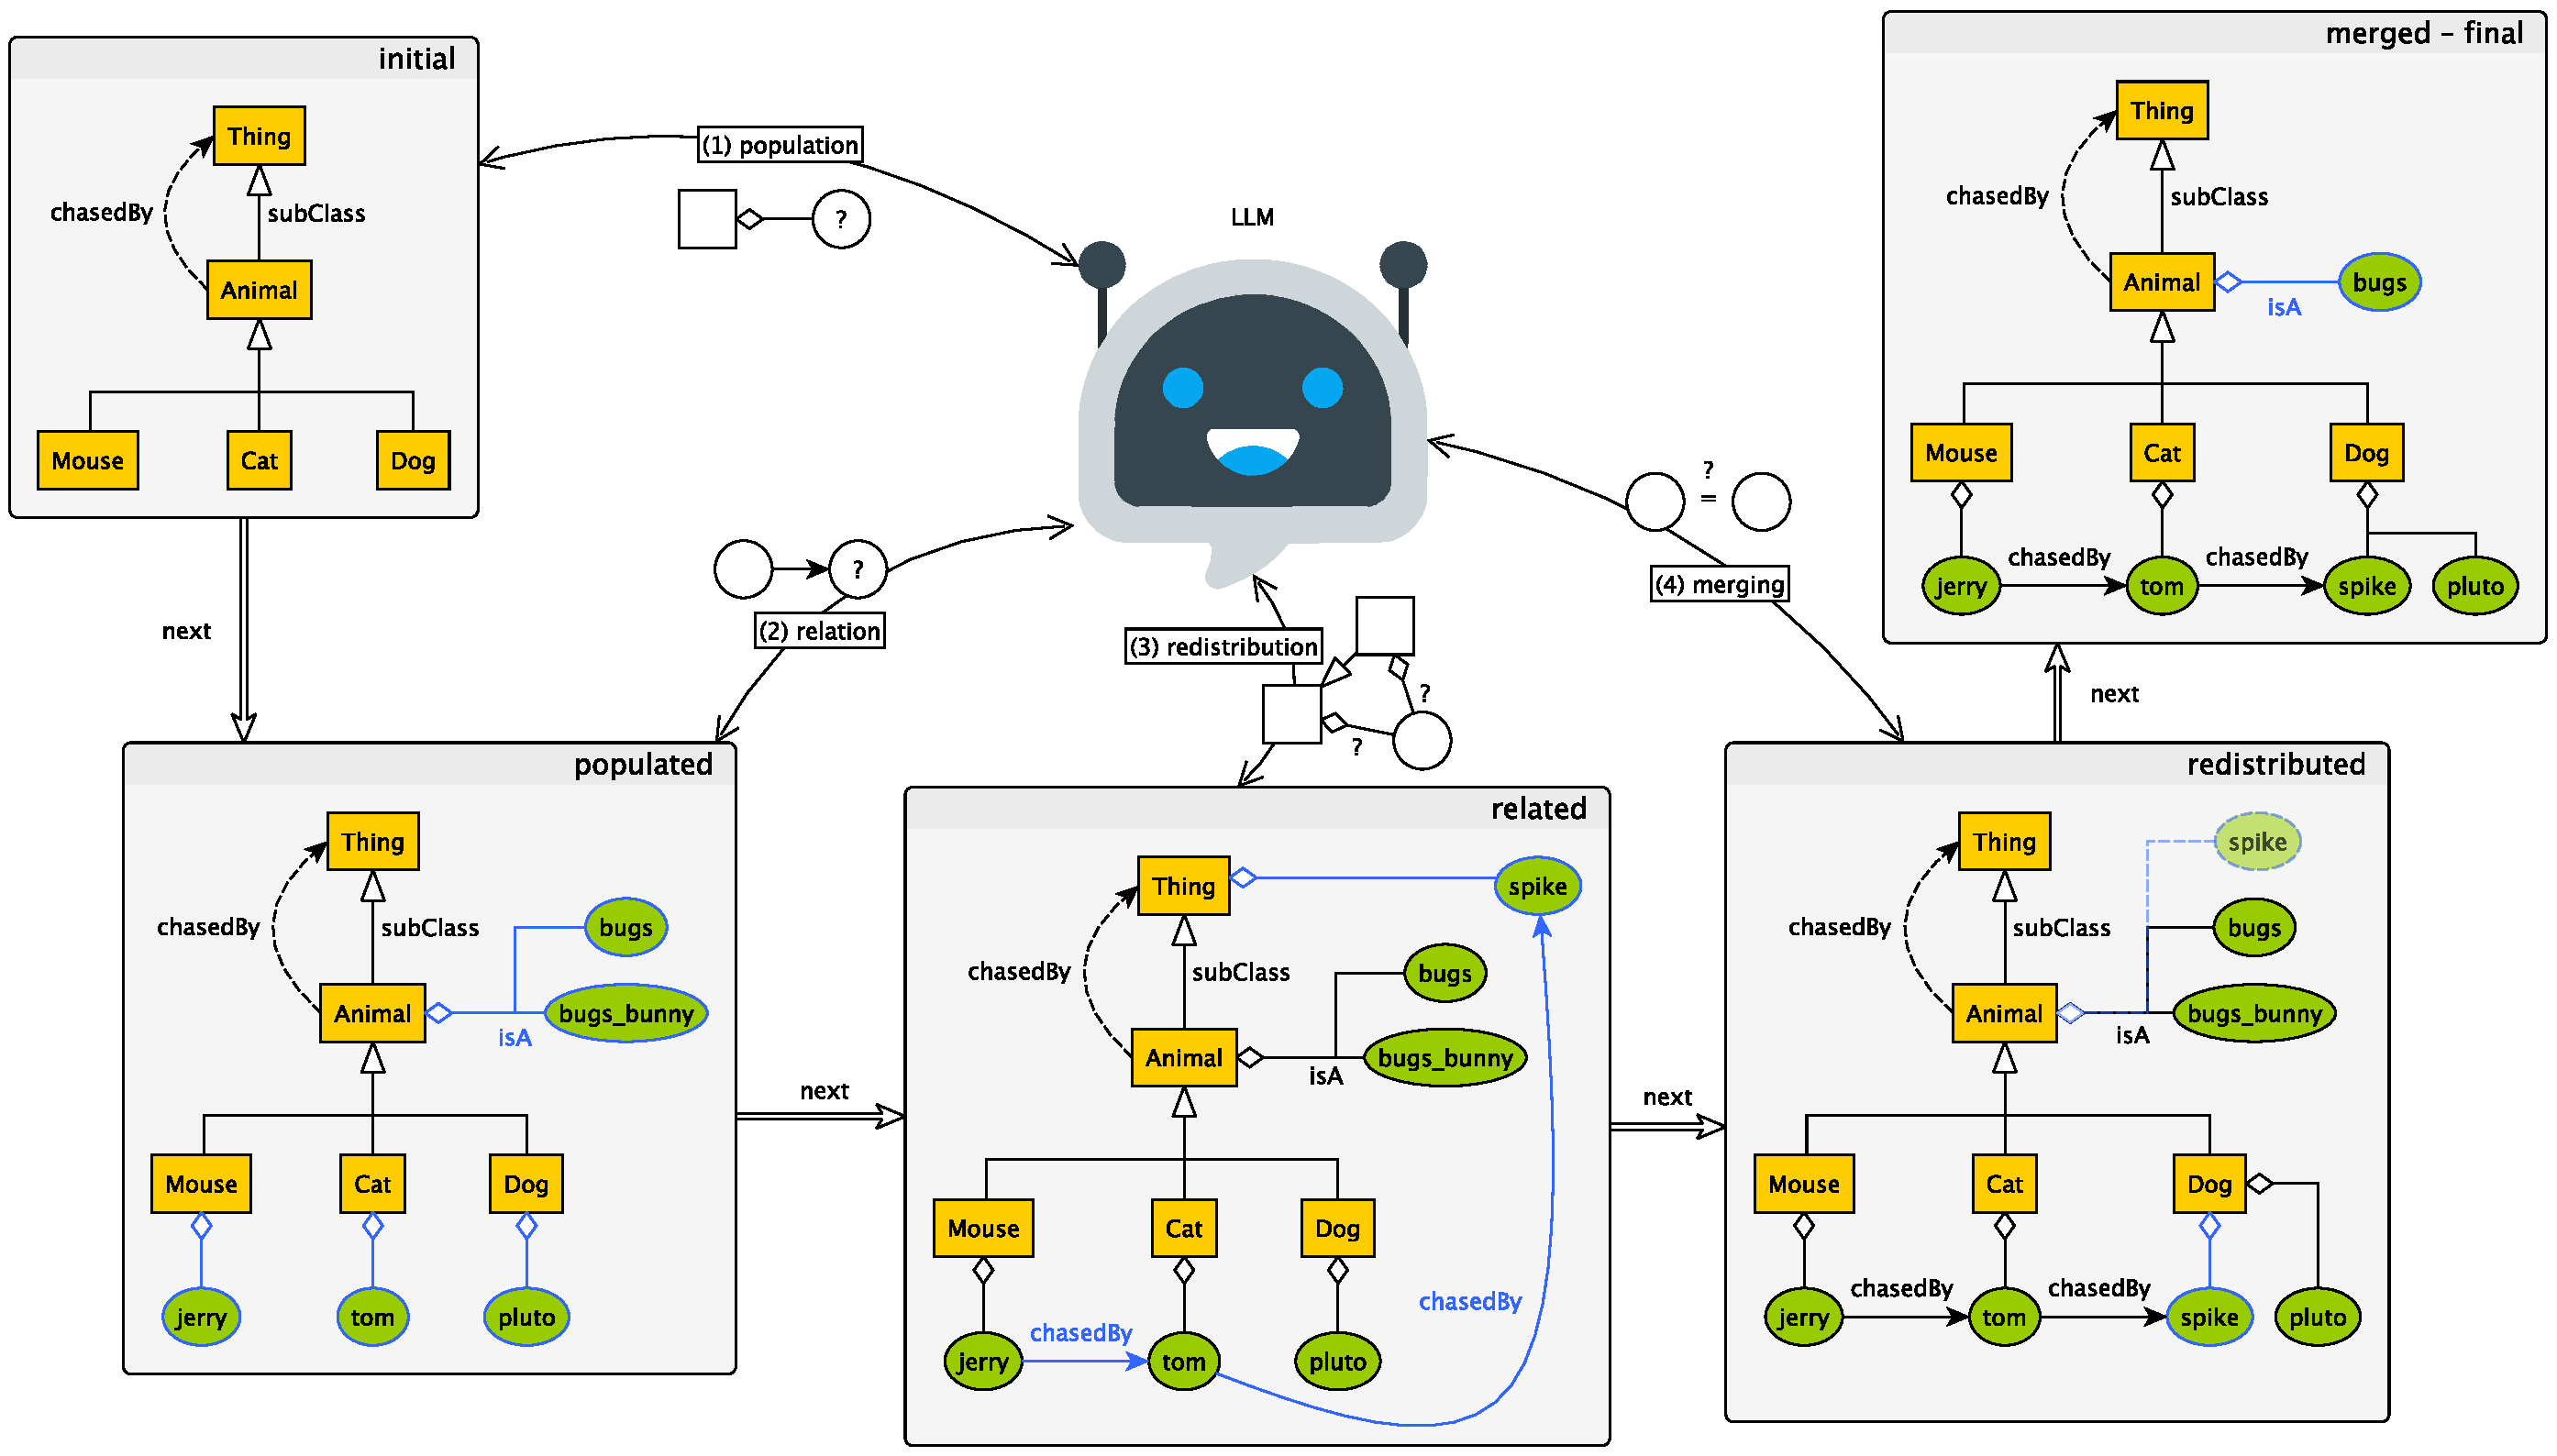
\includegraphics[width=\linewidth]{figures/kgfiller/roadmap}
    \caption[Overview of \llmfkg{}]{%
        Overview of \llmfkg{}, illustrated with a running example.
        %
        The example assumes an ontology about animals, including classes such as $\concept{Cat}$, $\concept{Dog}$, and $\concept{Mouse}$, which are subclasses of $\concept{Animal}$, itself a subclass of $\concept{Thing}$ (\(\top\)).
        %
        Initially, the ontology contains no instances.
        %
        A property $\relation{chasedBy} : \concept{Animal} \times \top$ is defined, indicating that animals can be chased by other entities.
        %
        The figure outlines the four phases of the \llmfkg{} algorithm, with changes highlighted in blue.
    }
    \label{fig:roadmap}
\end{figure}

The \llmfkg{} framework is designed for semi-automatic ontology population, leveraging \glspl{LLM} as oracles.
%
An overview of the \llmfkg{} framework is depicted in \Cref{fig:roadmap}.
%
This section provides a concise yet general description of the framework.

%
\paragraph{Core Functionality}
\label{par:core-functionality}

At its core, \llmfkg{} operates on a partially instantiated ontology.
%
The ontology must include class and property definitions, organized hierarchically as a directed acyclic graph (DAG).
%
Classes may or may not have instances.

%
Class names should be meaningful, concise, and unambiguous to avoid issues during query generation for the \gls{LLM}.
%
The same applies to property names.

%
Given these assumptions, \llmfkg{} generates individuals for all classes and associates them using the ontology's properties.
%
Generated individuals are assigned meaningful names and placed in the most specific class available.

%
The framework supports two primary use cases:
%
\begin{inlinelist}
    \item ontology designers have defined the ontology's structure but lack instances, and
    %
    \item designers want to add more instances to an already populated ontology.
\end{inlinelist}
%
These use cases can be combined, allowing iterative rounds of population and manual refinement.

%
\paragraph{Query Templates}
\label{par:query-templates}

\llmfkg{} relies on query templates to generate questions for the \gls{LLM}.
%
Templates are text strings containing placeholders, which are replaced with actual values during execution.
%
For example, the template \(t = \)\text{``What is the capital of \(\langle c \rangle\)?''} can be instantiated with the substitution \(\sigma = \{\langle c \rangle \mapsto \text{``Italy''}\}\), resulting in \(t / \sigma = \text{``What is the capital of Italy?''}\).

%
We define four types of query templates:
%
\begin{itemize}
    \item \textbf{Individual-seeking templates:} Ask for instances of a class, e.g., ``Examples of \(\langle \text{class} \rangle\)?''.
    %
    \item \textbf{Relation-seeking templates:} Ask for individuals related to a given individual via a property, e.g., ``Examples of \(\langle \text{property} \rangle\) for \(\langle \text{individual} \rangle\)?''.
    %
    \item \textbf{Best-match templates:} Ask for the best class for an individual among candidates, e.g., ``What class is best for \(\langle \text{individual} \rangle\) among \(\langle \text{classes} \rangle\)?''.
    %
    \item \textbf{Individuals-merging templates:} Ask if two instances in a class are identical, e.g., ``In \(\langle \text{class} \rangle\), are \(\langle \text{ind1} \rangle\) and \(\langle \text{ind2} \rangle\) the same?''.
\end{itemize}

%
\paragraph{\gls{LLM} Oracle}
We do not impose constraints on the nature of the \gls{LLM} oracle or the underlying model.
%
\texttt{KGFiller} is agnostic to the specific \gls{LLM} used, as long as it supports generating textual responses from textual prompts.
%
Both prompts and responses are assumed to be strings of arbitrary length, written in a natural language.
%
The natural language must match the one used for naming classes and properties in the ontology.
%
Without loss of generality, we assume this language is English.
%
A key assumption is that the \gls{LLM} oracle is pre-trained on a large corpus of textual data, which includes domain-specific knowledge relevant to the ontology.


\paragraph{Problem Statement}
We formalize the ontology population problem addressed by \texttt{KGFiller} as follows:
%
\begin{enumerate}
    \item A partially instantiated ontology \(\mathcal{O} = \mathcal{C} \cup \mathcal{P} \cup \mathcal{I}\), where:
    %
    \begin{itemize}
        \item \(\mathcal{C} \neq \emptyset\) is a non-empty set of class definitions,
        \item \(\mathcal{P} \neq \emptyset\) is a non-empty set of property definitions, and
        \item \(\mathcal{I}\) is a possibly empty set of individuals and their relationships.
    \end{itemize}
    %
    \item A subsumption relation \(\sqsubseteq\) among the classes in \(\mathcal{C}\).
    %
    \item A set of query templates \(\mathcal{T} = \mathcal{T}_I \cup \mathcal{T}_R \cup \mathcal{T}_B \cup \mathcal{T}_M\), where:
    %
    \begin{itemize}
        \item \(\mathcal{T}_I\) contains individual-seeking templates,
        \item \(\mathcal{T}_R\) contains relation-seeking templates,
        \item \(\mathcal{T}_B\) contains best-match templates, and
        \item \(\mathcal{T}_M\) contains individuals-merging templates.
    \end{itemize}
    %
    \item A trained \gls{LLM} oracle \(\mathcal{L}\), encapsulating domain-specific knowledge.
\end{enumerate}

%

The goal of \texttt{KGFiller} is to generate a set of individuals and relationships \(\mathcal{I}'\) such that \(\mathcal{I} \subseteq \mathcal{I}'\).
%
All new individuals and relationships in \(\mathcal{I}'\) must be consistent with the class and property definitions in \(\mathcal{C}\) and \(\mathcal{P}\), respectively.
%
Specifically:
%
\begin{itemize}
    \item Every individual is associated with the most specific concept in \(\mathcal{C}\) with respect to \(\sqsubseteq\).
    %
    \item For every property in \(\mathcal{P}\), every individual in the property’s domain is associated with one or more individuals in the property’s range.
\end{itemize}


\paragraph{Phases}
To compute \(\mathcal{I}'\), \texttt{KGFiller} executes four sequential phases:
%
\begin{enumerate}
    \item \textbf{Population Phase:} Novel individuals are identified for each class in \(\mathcal{C}\).
    %
    \item \textbf{Relation Phase:} New relationships are identified for each property in \(\mathcal{P}\).
    %
    \item \textbf{Redistribution Phase:} Individuals are redistributed among the classes in \(\mathcal{C}\) to ensure each individual is placed in the most specific class available.
    %
    \item \textbf{Merge Phase:} Semantic duplicates within each class in \(\mathcal{C}\) are detected and merged.
\end{enumerate}
%
The order of these phases is critical.
%
The population phase generates individuals used in the relation phase, which may, in turn, generate additional individuals.
%
The redistribution phase ensures all individuals are placed in the most specific class, while the merge phase reduces semantic duplication.


\paragraph{Ancillary functions}
%
The next section introduces several auxiliary functions used throughout the framework.
%
The function \texttt{GetRange} (resp., \texttt{GetDomain}) retrieves the range (resp., domain) of a given property.
%
The function \texttt{AskOracle} models queries to the \gls{LLM} oracle, accepting and returning arbitrary strings.
%
The function \texttt{ExtractBinary} (resp., \texttt{ExtractNames}) extracts binary values (resp., relevant names of individuals or concepts) from the textual responses of the \gls{LLM}.
%
It returns a Boolean value (resp., a list of names) and accepts a string as input.
%
Finally, the function \texttt{AddToClass} assigns an individual to a class.
%
If the individual is already part of the class or any of its subclasses, the function performs no action.


\subsubsection{Population Phase}
\label{subsubsec:population-phase}
%
\begin{algorithm}
    \captionsetup{font=\algCaptionSize}
    \caption{Populates the given ontology with novel individuals queried from an LLM oracle}
    \label{alg:populate}
    \begin{algorithmic}[1]\algCodeSize
        \Require $\relset{O} = \relset{C} \cup \relset{P} \cup \relset{X}$: partially populated ontology
        \Require $\relset{T}_{I}$: individual seeking query templates
        \Require $\relset{L}$: LLM oracle
        \Require $\concept{R} \in \relset{C}$: root concept to be populated
        \Ensure $\relset{X}'$ contains novel individuals, assigned to the classes in $\relset{C}$
        \medskip
        \Function{\populate}{$\relset{O}, \relset{T}_I, \relset{L}, \concept{R}$}
            \State $\relset{X}' \gets \relset{X}$
            \ForAll{$\concept{C} \in \relset{C} \suchThat \concept{C} \sqsubset \concept{R} \wedge \concept{C} \neq \bot$}
                \State $\relset{O}' \gets \relset{C} \cup \relset{P} \cup \relset{X}'$
                \State $\relset{X}' \gets \Call{\populate}{\relset{O}', \relset{T}_{I}, \relset{L}, \concept{C}}$
            \EndFor
            \ForAll{$\mathit{t} \in \relset{T}_{I}$}
                \State $\mathit{q} \gets \mathit{t}/\{ \var{class} \mapsto \concept{R} \}$
                \State $\mathit{text} \gets \Call{\askOracle}{\relset{L}, \mathit{q}}$
                \ForAll{$\instance{i} \in \Call{\extractNames}{\mathit{text}}$}
                    \State $\relset{O}' \gets \relset{C} \cup \relset{P} \cup \relset{X}'$
                    \State $\relset{X}' \gets \Call{\addToClass}{\relset{O}', \instance{i}, \concept{R}}$
                \EndFor
            \EndFor
            \State \Return $\relset{X}'$
        \EndFunction
    \end{algorithmic}
\end{algorithm}
%
The population phase is based on the \populate{} function, as defined in \Cref{alg:populate}.
%
This function is designed to populate a partially instantiated ontology, denoted as $\relset{O}$, with new instances.
%
It achieves this by querying a \gls{LLM} oracle, represented as $\relset{L}$, using a set of instance-seeking query templates, $\relset{T}_{I}$.


The process begins with a root class $\concept{R} \in \relset{O}$.
%
The function then traverses the class hierarchy defined by the subsumption relation $\sqsubseteq$, following a depth-first post-order strategy.
%
This means that all direct and indirect subclasses of $\concept{R}$ are visited before $\concept{R}$ itself, ensuring that the most specific classes are populated first.
%
Such a strategy is crucial to guarantee that any individual generated during this phase is assigned to the most specific class available.


For each subclass $\concept{C} \sqsubseteq \concept{R}$, the function generates queries by replacing the placeholder $\var{class}$ in each template from $\relset{T}_{I}$ with the name of $\concept{C}$.
%
These queries are then submitted to the \gls{LLM} oracle $\relset{L}$, and the responses are processed to extract the names of the individuals.
%
The number of individuals generated per query is unbounded and depends on the capabilities of the \gls{LLM} oracle $\relset{L}$ and other implementation-specific factors.


It is possible for the same individual to be generated by multiple queries or for multiple subclasses of $\concept{R}$.
%
However, this does not pose any issues, as the \addToClass{} function ensures that individuals are not duplicated and are always assigned to the most specific class.
%
This behavior aligns with the post-order exploration strategy, which prioritizes the population of specific concepts over more general ones.


To populate the entire ontology $\relset{O}$, the function can be invoked with the top class $\top$ as the root:
%
\Call{\populate}{$\relset{O}, \relset{T}_I, \relset{L}, \top$}.
%
This ensures that all classes in $\relset{O}$ are visited and populated systematically.


\subsubsection{Relation Phase}
\label{subsubsec:relation-phase}
%
\begin{algorithm}
    \captionsetup{font=\algCaptionSize}
    \caption{Populates the given ontology with novel relationships queried from an LLM oracle}
    \label{alg:relate}
    \begin{algorithmic}[1]\algCodeSize
        \Require $\relset{O} = \relset{C} \cup \relset{P} \cup \relset{X}$: partially populated ontology
        \Require $\relset{T}_{R}$: relation seeking query templates
        \Require $\relset{L}$: LLM oracle
        \Require $\relation{P} \in \relset{P}$: property to be populated
        \Ensure $\relset{X}'$ contains novel relationships, involving individuals in $\relset{X}$
        \medskip
        \Function{\relate}{$\relset{O}, \relset{T}_R, \relset{L}, \relation{P}$}
            \State $\relset{X}' \gets \relset{X}$
            \State $\concept{D} \gets \Call{\getDomain}{\relation{P}}$
            \State $\concept{R} \gets \Call{\getRange}{\relation{P}}$
            \ForAll{$(\instance{i} : \concept{D}) \in \relset{X}$}
                \ForAll{$\mathit{t} \in \relset{T}_{R}$}
                    \State $\mathit{q} \gets \mathit{t}/\{ \var{individual} \!\mapsto\! \instance{i}, \var{property} \!\mapsto\! \relation{P} \}$
                    \State $\mathit{text} \gets \Call{\askOracle}{\relset{L}, \mathit{q}}$
                    \ForAll{$\instance{i}' \in \Call{\extractNames}{\mathit{text}}$}
                        \State $\relset{O}' \gets \relset{C} \cup \relset{P} \cup \relset{X}'$
                        \State $\relset{X}' \gets \Call{\addToClass}{\relset{O}', \instance{i}', \concept{R}}$
                        \State $\relset{X}' \gets \relset{X}' \cup \{ \relation{P}(\instance{i}, \instance{i}') \}$
                    \EndFor
                \EndFor
            \EndFor
            \State \Return $\relset{X}'$
        \EndFunction
    \end{algorithmic}
\end{algorithm}
%
The relation phase utilizes the \relate{} function to populate a partially instantiated ontology, \(\relset{O}\), with new relationships.
%
These relationships link existing individuals and may introduce novel individuals, based on queries to a \gls{LLM} oracle, \(\relset{L}\), using a set of relation-seeking query templates, \(\relset{T}_{R}\).

%
Consider a property \(\relation{p} \in \relset{O}\), defined as \(\relation{p} : \concept{D} \times \concept{R}\), where \(\concept{D}\) and \(\concept{R}\) represent the domain and range of \(\relation{p}\), respectively.
%
The function queries the \gls{LLM} oracle, \(\relset{L}\), to identify relationships between each individual \(\instance{i} \in \concept{D}\) and potential individuals \(\instance{i}' \in \concept{R}\) through \(\relation{p}\).

%
For each individual \(\instance{i}\) and each query template \(t \in \relset{T}_{R}\), a query \(q\) is generated by substituting placeholders \(\var{property}\) and \(\var{individual}\) in \(t\) with the names of \(\relation{p}\) and \(\instance{i}\), respectively.
%
The query \(q\) is submitted to the \gls{LLM} oracle, and the response is processed to extract the names of individuals to be added to the ontology.
%
Each new individual \(\instance{i}'\) is added to the range \(\concept{R}\) of \(\relation{p}\), along with the relationship \(\relation{p}(\instance{i}, \instance{i}')\).

%
To populate relationships for all properties \(\relation{p} \in \relset{O}\), the function is invoked for each property as follows:
%
\Call{\relate}{$\relset{O}, \relset{T}_R, \relset{L}, \relation{p}$}.

%
It is important to note that the \relate{} function may generate new individuals during its execution.
%
In some cases, the range \(\concept{R}\) of the property \(\relation{p}\) may not be the most specific class for these individuals.
%
For example, a subclass \(\concept{C} \sqsubset \concept{R}\) might better represent some of the generated individuals.
%
This necessitates the redistribution phase, which ensures that all individuals are assigned to the most specific class available.


\subsubsection{Redistribution Phase}
\label{subsubsec:redistribution-phase}
%
\begin{algorithm}
    \captionsetup{font=\algCaptionSize}
    \caption{Redistributes individuals from the given ontology's classes, in such a way that each individual is assigned to the most specific class available}
    \label{alg:redistribute}
    \begin{algorithmic}[1]\algCodeSize
        \Require $\relset{O} = \relset{C} \cup \relset{P} \cup \relset{X}$: partially populated ontology
        \Require $\relset{T}_{B}$: relation seeking query templates
        \Require $\relset{L}$: LLM oracle
        \Require $\concept{R} \in \relset{C}$: root concept within which redistribution should occur
        \Ensure $\relset{X}'$ contains the different assignments of individuals to classes
        \medskip
        \Function{\redistribute}{$\relset{O}, \relset{T}_B, \relset{L}, \concept{R}$}
            \State $\relset{X}' \gets \relset{X}$
            \State $\relset{S} \gets \{ \concept{S} \in \relset{C} \mid \concept{S} \sqsubset \concept{R} \}$
            \ForAll{$(\instance{i} : \concept{R}) \in \relset{X}'$}
                \State $\concept{B} \gets \concept{R}$
                \ForAll{$\mathit{t} \in \relset{T}_{B}$}
                    \State $\mathit{q} \gets \mathit{t}/\{ \var{individual} \mapsto \instance{i}, \var{classes} \mapsto \relset{S} \}$
                    \State $\mathit{text} \gets \Call{\askOracle}{\relset{L}, \mathit{q}}$
                    \ForAll{$\concept{C} \in \Call{\extractNames}{\mathit{text}}$}
                        \State $\concept{B} \gets \concept{C}$
                        \State \Break{going to line \ref{line:first-result}}
                    \EndFor
                \EndFor
                \State $\relset{O}' \gets \relset{C} \cup \relset{P} \cup \relset{X}'$ \label{line:first-result}
                \State $\relset{X}' \gets \Call{\addToClass}{\relset{O}', \instance{i}, \concept{B}}$
            \EndFor
            \ForAll{$\concept{C} \in \relset{C} \suchThat \concept{C} \sqsubset \concept{R} \wedge \concept{C} \neq \bot$}
                \State $\relset{O}' \gets \relset{C} \cup \relset{P} \cup \relset{X}'$
                \State $\relset{X}' \gets \Call{\redistribute}{\relset{O}', \relset{T}_{B}, \relset{L}, \concept{C}}$
            \EndFor
            \State \Return $\relset{X}'$
        \EndFunction
    \end{algorithmic}
\end{algorithm}
%
The redistribution phase utilizes the \redistribute{} function, as defined in \Cref{alg:redistribute}.
%
This function redistributes individuals among the classes of an instantiated ontology, \(\relset{O}\), ensuring that each individual is assigned to the most specific class available.
%
To achieve this, the function queries the \gls{LLM} oracle, \(\relset{L}\), using a set of best-match query templates, \(\relset{T}_{B}\).

%
Starting from a root class \(\concept{R} \in \relset{O}\), the function recursively explores the class hierarchy defined by the subsumption relation \(\sqsubseteq\).
%
It follows a depth-first pre-order traversal strategy, visiting each class before its subclasses.
%
This approach ensures that individuals can be reassigned to more specific classes as the traversal progresses.

%
For each visited class \(\concept{C} \sqsubseteq \concept{R}\), the function evaluates whether \(\concept{C}\) is the most appropriate class for all individuals currently assigned to it.
%
If a more specific subclass of \(\concept{C}\) is better suited for an individual, the function reassigns the individual accordingly.
%
For example, if \(\concept{Cat} \sqsubset \concept{Animal}\) and an individual \(\instance{tom}\) is initially assigned to \(\concept{Animal}\), the function reassigns \(\instance{tom}\) to \(\concept{Cat}\).

%
To determine the best class for an individual \(\instance{i} : \concept{C}\), the function generates a query for each template \(t \in \relset{T}_{B}\).
%
The placeholders \(\var{individual}\) and \(\var{classes}\) in \(t\) are replaced with the name of \(\instance{i}\) and the concatenated names of all direct subclasses of \(\concept{C}\), respectively.
%
The resulting query is submitted to the \gls{LLM} oracle, and the response is processed to extract candidate class names.
%
The first class in the response is selected as the best match, and \(\instance{i}\) is reassigned to it.

%
Since the function is recursive, an individual may be reassigned multiple times until it reaches the most specific class available in the ontology.
%
The depth-first pre-order strategy is crucial for this process, as it allows individuals to ``move down'' the class hierarchy efficiently while keeping query sizes manageable.

%
To redistribute all individuals in an ontology, the function can be invoked with the top class \(\top\) as the root:
%
\Call{\redistribute}{$\relset{O}, \relset{T}_{B}, \relset{L}, \top$}.
%
This ensures that every individual in \(\relset{O}\) is assessed and reassigned to the most specific class, if necessary.


\subsubsection{Merge Phase}
\label{subsubsec:merge-phase}
%
\begin{algorithm}
    \captionsetup{font=\algCaptionSize}
    \caption{Merges syntactically and semantically similar individuals from the given ontology's classes}
    \label{alg:merge}
    \begin{algorithmic}[1]\algCodeSize
        \Require $\relset{O} = \relset{C} \cup \relset{P} \cup \relset{X}$: partially populated ontology
        \Require $\relset{T}_{M}$: indivuals merging query templates
        \Require $\relset{L}$: LLM oracle
        \Require $\concept{R} \in \relset{C}$: root concept within which merge should occur
        \Ensure $\relset{X}'$ contains no duplicated individuals
        \medskip
        \Function{\merge}{$\relset{O}, \relset{T}_{M}, \relset{L}, \concept{R}$}
            \State $\relset{X}' \gets \relset{X}$
            \ForAll{$\concept{C} \in \relset{C} \suchThat \concept{C} \sqsubset \concept{R}$}
                \State $\mathcal{D} \gets \emptyset$
                \ForAll{$\instance{i}, \instance{j} : \concept{C} \suchThat ( \instance{i}, \instance{j} ) \in \relset{X}' \times \relset{X}'$}
                    \If{$\Call{\synSimilar}{\instance{i}, \instance{j}}$}
                        \State $\mathcal{D} \gets \mathcal{D} \cup \{\{\instance{i}, \instance{j}\}\}$
                    \EndIf
                \EndFor
                \ForAll{$\{ \instance{i}, \instance{j} \} \in \mathcal{D}$}
                    \ForAll{$\mathit{t} \in \relset{T}_{M}$}
                    \label{line:next-couple}
                        \State $\mathit{q} \gets \mathit{t}/\{ \var{ind_1}\!\mapsto\!\instance{i}, \var{ind_2}\!\mapsto\!\instance{j},
                            \var{class}\!\mapsto\!\concept{C} \}$
                        \State $\mathit{text} \gets \Call{\askOracle}{\relset{L}, \mathit{q}}$
                        \If{$\Call{\extractBinary}{text}$}
                            \State $\relset{X}' \gets \Call{\mergeInst}{i, j}$
                            \State \Break{going to line \ref{line:next-couple}}
                        \EndIf
                    \EndFor
                \EndFor
            \EndFor
        \EndFunction
    \end{algorithmic}
\end{algorithm}

%
The \merge{} function is responsible for identifying and merging duplicated individuals in an instantiated ontology, denoted as $\relset{O}$.
%
Duplicated individuals are defined as those with slightly different names but representing the same semantic entity.
%
Such duplicates often arise as a by-product of earlier phases in the ontology population process.


For example, consider the individuals $\instance{maincoone\_cat}$ and $\instance{maincoone}$, both belonging to the class $\concept{Cat} \sqsubset \concept{Animal}$.
%
Although their names differ syntactically, they refer to the same entity.
%
To address this, the \merge{} function queries the \gls{LLM} oracle, denoted as $\relset{L}$, to identify semantically similar individuals and merge them into a single entity.


The \merge{} function operates by scanning the ontology $\relset{O}$ for pairs of syntactically similar individuals.
%
For each pair, it uses a set of merging query templates, $\relset{T}_{M}$, to query the \gls{LLM} oracle.
%
The oracle's response determines whether the individuals should be merged.


The process begins with a root class $\concept{R} \in \relset{O}$ and recursively explores the class hierarchy defined by the subsumption relation $\sqsubseteq$.
%
For each class $\concept{C} \sqsubseteq \concept{R}$, the function identifies a set $\mathcal{D}$ of candidate duplicate pairs using the \synSimilar{} function.
%
Each pair is then evaluated using the \extractBinary{} function, which interprets the oracle's response as a Boolean value.
%
If the response is positive, the \mergeInst{} function is invoked to merge the individuals.
%
This involves transferring all information from one individual to the other and removing the redundant individual, resulting in an updated ontology $\relset{X}'$.


The merging process relies on templates in $\relset{T}_{M}$.
%
For each candidate pair, a query is generated by replacing the placeholders $\var{ind\_1}$, $\var{ind\_2}$, and $\var{class}$ in the template with the names of the individuals and the class $\concept{C}$, respectively.
%
The first template yielding a positive response is considered definitive, and further templates are not queried.
%
To ensure deterministic behavior and avoid issues arising from the oracle's creativity, the temperature parameter is set to 0.0 during these queries.


To detect and merge all duplicated individuals in an ontology $\relset{O}$, the function can be invoked as follows:
%
\Call{\merge}{$\relset{O}, \relset{T}_M, \relset{L}, \top$}.
%
This ensures that all classes in $\relset{O}$ are systematically visited, and any semantic duplicates are resolved.


\paragraph{Remarks}
%
\Cref{alg:merge} employs a post-order exploration strategy.
%
However, the choice of exploration strategy is \emph{not} critical for the merging phase.
%
Alternative strategies can be used, provided they visit all direct and indirect subclasses of $\concept{R}$.

%
The \synSimilar{} function plays a crucial role in determining whether two instances, $\instance{i}$ and $\instance{j}$, are sufficiently similar to be considered for merging.
%
Its implementation significantly impacts the overall performance of the \merge{} function.
%
% For example, one could define similarity based on shared substrings longer than a threshold $\lambda$.
% %
% Empirically, $\lambda$ can be set to 4 characters.

%
Regarding the merging phase, one might question why entity alignment approaches~\cite{ZhaoTkde2022} are not used.
%
While effective for identifying similar instances across different \glspl{KG}, these methods typically require additional domain-specific data~\cite{ChenIjcai2018,XuAcl2019}.
%
This is because entity alignment systems rely on ad-hoc \gls{ML} models trained for the alignment task, introducing extra complexity.

%
In contrast, our approach leverages the same \gls{LLM} oracle for both ontology population and duplicate identification.
%
Although not entirely error-free, this method avoids additional computational overhead during the population phase.
%
It also eliminates the need for users to provide extra domain-specific data or train additional models, simplifying the overall process.
%



\subsection{Case Study and Experiments}
\label{subsec:case-study}
%
This section presents a case study designed to empirically validate \llmfkg{}.

%
\subsubsection{Experimental Setup}
\label{subsubsec:experimental-setup}
%
The experimental setup involves designing a non-trivial ontology, as detailed in \Cref{subsubsec:kgfiller-ontology}.
%
The ontology includes a class hierarchy and a set of properties, which are populated using \llmfkg{}.
%
We fine-tune specific query templates (\Cref{subsubsec:query-templates}) and utilize various \glspl{LLM} from different families and technologies (\Cref{subsubsec:llms-oracles}).
%
This process generates a set of populated ontologies, all sharing the same structure but differing in their content.
%
The populated ontologies are analyzed and compared to evaluate the performance of \llmfkg{} and the impact of the chosen \gls{LLM} on the quality of the population process.
%
To achieve this, we define a taxonomy of errors and a set of metrics (\Cref{subsec:performance-metrics}) to measure the quality of the generated ontologies.
%
The evaluation is performed through a manual inspection of the populated ontologies, examining each individual and relationship (\Cref{subsec:results}).

%
Testing \llmfkg{} on a custom ontology, rather than a publicly available one, offers several advantages.
%
First, it allows precise control over the experiment's complexity and content.
%
Second, it avoids potential biases where \glspl{LLM} perform well due to prior exposure to the ontology during training.
%
However, this approach lacks ground truth data, making automatic validation infeasible.
%
Thus, manual inspection is necessary to identify errors and ensure the correctness of the algorithm's output.

%
\subsubsection{Code and Data}
\label{subsubsec:code-and-data}
%
The experiments are conducted using a Python implementation of \llmfkg{}, which is publicly available on GitHub\footnote{\url{https://github.com/Chistera4-Expectation/kg-filler}}.
%
The experimental results are also available on a dedicated repository\footnote{\url{https://github.com/Chistera4-Expectation/knowledge-graphs/branches}}, where each Git branch corresponds to a specific experiment.
%
The \texttt{main} branch contains the initial ontology, which includes only class and property definitions without any individuals.

%
For reproducibility, each experiment branch includes the populated ontology and the cache of query--response pairs from the \gls{LLM}.
%
This allows others to inspect the exact queries and responses and reproduce the experiments deterministically.
%
Additionally, the experiments are automated, with each commit in the branch corresponding to a single operation performed by \llmfkg{} (e.g., populating a class or property).
%
This commit history provides a detailed sequence of operations for each experiment.

%
\subsubsection{Ontology}
\label{subsubsec:kgfiller-ontology}
%
\begin{figure*}
    \centering
    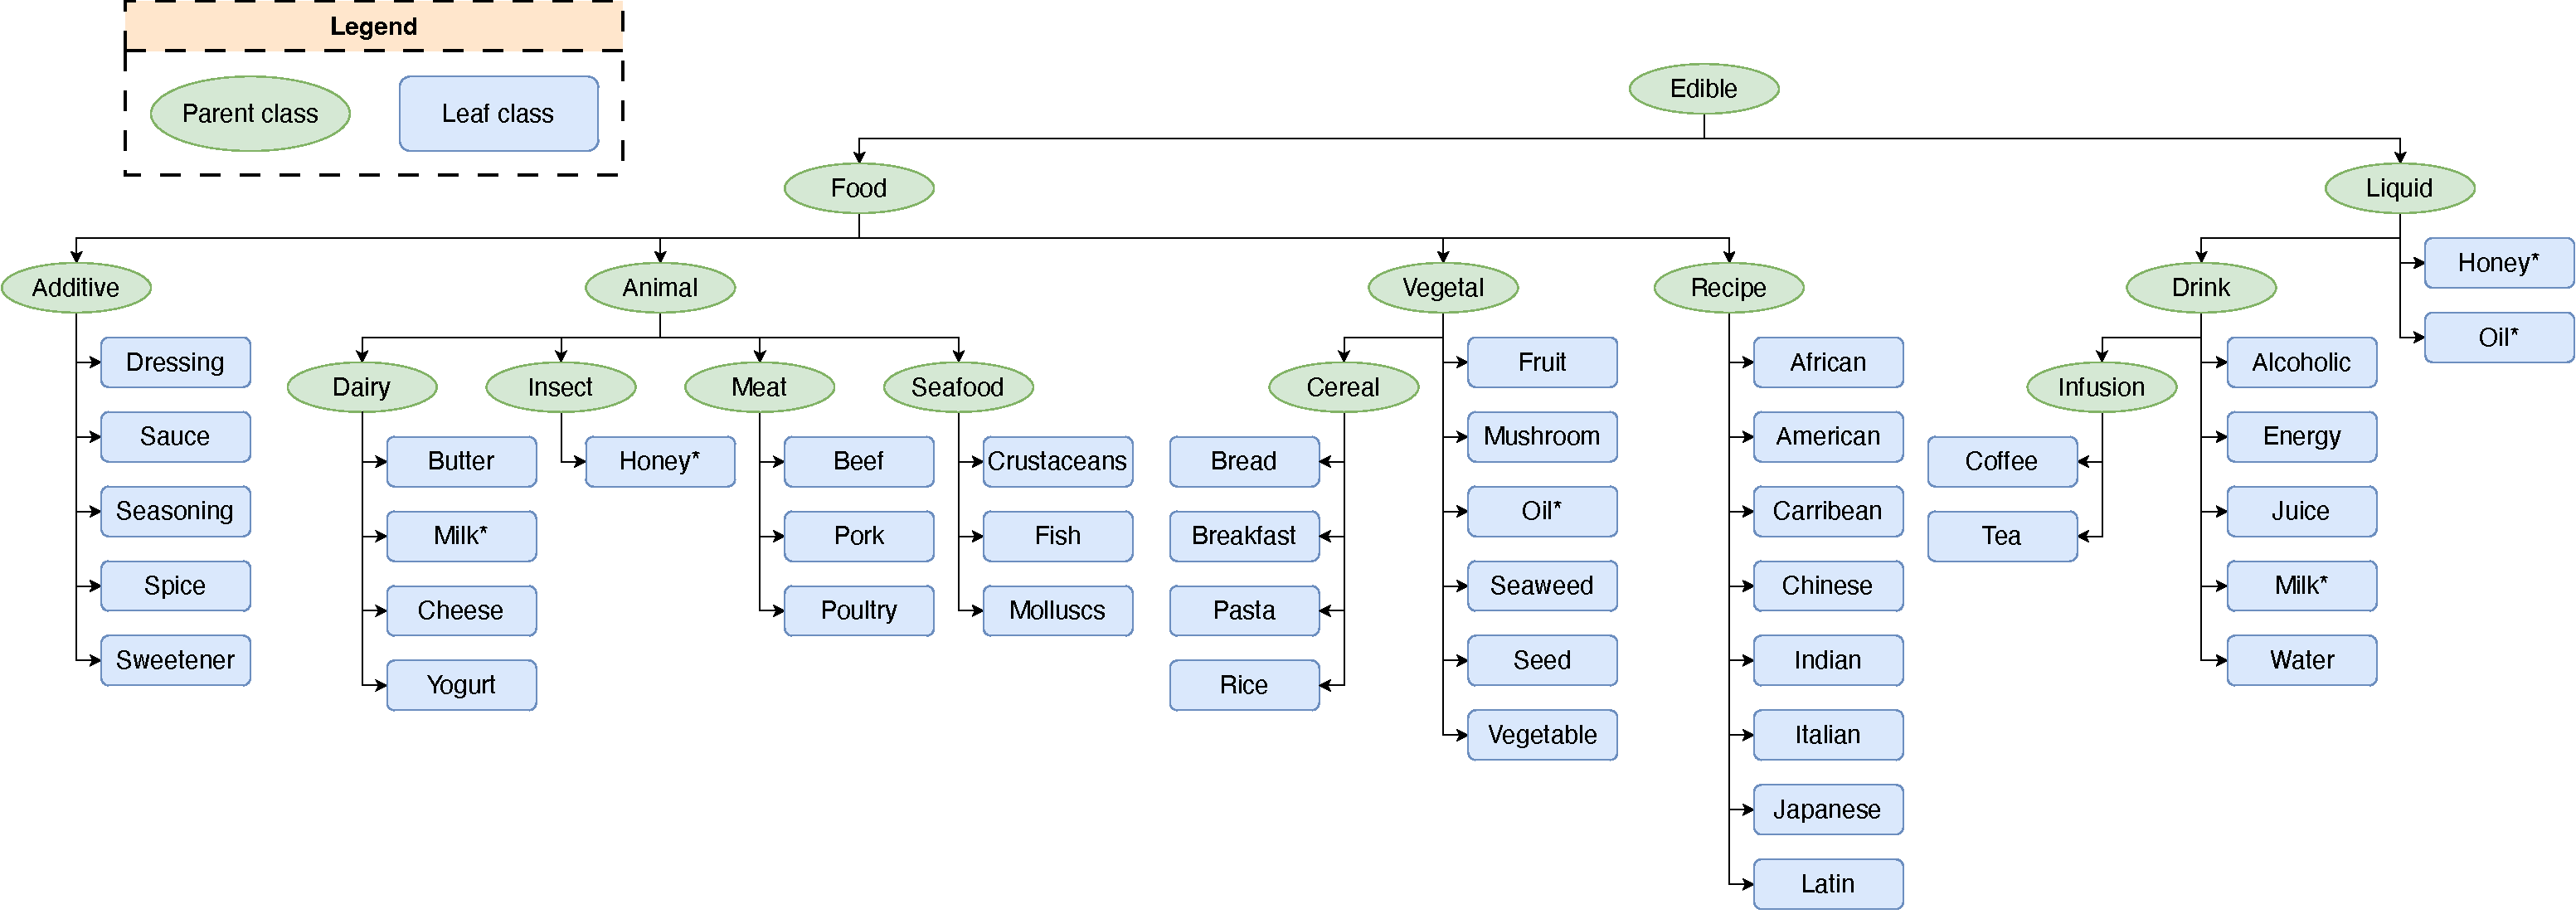
\includegraphics[width=\linewidth]{figures/kgfiller/ontology-skeleton}
    \caption[Class hierarchy of the ontology used in the experiments]{
        %
        Class hierarchy of the case study ontology.
        %
        Notice that the hierarchy is not really a tree, but rather a \gls{DAG}.
        %
        The asterisk (*) denotes classes having multiple super-classes (they are depicted once per super-class for the sake of readability).
    }
    \label{fig:ontology}
\end{figure*}
%
The ontology is designed in the \emph{nutritional} domain, as required by the \expectation{} project~\cite{expectation-extraamas2021}.
%
In \expectation{}, the ontology serves as the foundation for a nutritional recommender system, which suggests recipes based on users' dietary needs and preferences~\cite{DBLP:journals/cmpb/MagniniCCAO23}.
%
Although the recommender system is outside the scope of this work, this context helps clarify the ontology design choices.

%
The ontology focuses on representing \emph{recipes} and their \emph{ingredients}.
%
It categorizes \emph{edible} items into several subclasses to accommodate diverse dietary requirements and preferences.
%
\Cref{fig:ontology} illustrates the class hierarchy, which is structured as a directed acyclic graph (DAG).
%
The root class is \concept{Edible}, with subclasses such as \concept{Recipe}, which further branches into various cuisines (e.g., \concept{Italian}, \concept{Chinese}).

%
Some classes include an annotation property, \relation{fancyName}, to provide a more descriptive label for the class.
%
Another key property is $\relation{ingredientOf} : \concept{Edible} \times \concept{Recipe}$, which links recipes to their ingredients.
%
Initially, the ontology is a skeleton containing no individuals.

%
\subsubsection{Query Templates}
\label{subsubsec:query-templates}
%
To query the \gls{LLM} oracle, we define and fine-tune specific query templates.

%
The set of individual-seeking templates, $\relset{T}_{I}$, is defined as:
%
\str{$ ( $instances$ \mid $examples$ ) $ list for class $\var{class} ( $, names only$ )? $}.
%
Here, $(A|B)$ denotes two template variants, one with $A$ and one with $B$, while $(A)?$ indicates optional inclusion of $A$.

%
The set of relation-seeking templates, $\relset{T}_{R}$, includes:
%
\str{ingredient list for $\var{individual}$, names only}.
%
This template uses a hard-coded property name for natural phrasing.

%
The set of best-match templates, $\relset{T}_{B}$, is defined as:
%
\str{most adequate class for $\var{individual}$ among: $\var{classes}$. concise}.

%
Finally, the set of individual-merging templates, $\relset{T}_{M}$, is:
%
\str{in the $\var{class}$ class, should instances $\var{ind_1}$ and $\var{ind_2}$ be merged together as semantic and ontologic duplicates? yes or no answer only}.

%
\subsubsection{\gls{LLM} Oracles}
\label{subsubsec:llms-oracles}
%
To evaluate the impact of \gls{LLM} quality on \llmfkg{}, we integrate several state-of-the-art \glspl{LLM}.
%
These include both open-source models (e.g., OpenChat, Llama) and closed-source models (e.g., GPT), as well as \gls{MoE} models like Mixtral.

%
Open-source models are queried using the Hugging Chat API\footnote{\url{https://github.com/Soulter/hugging-chat-api}}, a third-party library for the HuggingFace platform\footnote{\url{https://huggingface.co}}.
%
This API supports multiple simultaneous conversations with different \glspl{LLM}.
%
The selected open-source models include:
%
\begin{description}
    \item[Llama 2:] A family of open-source \glspl{LLM}, with the 70 billion parameters model used in our experiments~\cite{llama2}.
    %
    \item[OpenChat 3.5:] A 13 billion parameters model fine-tuned from the Llama family, optimized for mixed-quality data~\cite{wang2023openchat}.
    %
    \item[Mistral 7B:] A 7 billion parameters model, designed for high performance relative to its size~\cite{mistral}.
    %
    \item[Gemma:] A lightweight model from Google, based on the Gemini research~\cite{gemini}.
\end{description}

%
For \gls{MoE} models, we include:
%
\begin{description}
    \item[Mixtral:] A sparse \gls{MoE} aggregating eight 7 billion parameters models~\cite{mixtral}.
    %
    \item[Nous Hermes:] A flagship model trained on high-quality data, including GPT-4 outputs.
\end{description}

%
Closed-source models are queried using the OpenAI API\footnote{\url{https://openai.com/blog/openai-api}}.
%
The selected models include:
%
\begin{description}
    \item[GPT 3.5 Turbo:] A widely used model with significant performance improvements~\cite{gpt3-2020}.
    %
    \item[GPT 4 Turbo:] The latest version, reported to be a \gls{MoE}~\cite{gpt4}.
\end{description}

%
\Cref{tab:llms_sizes} summarizes the \glspl{LLM} used, their sizes, and relevant hyperparameters.
%
The size of the \gls{LLM} significantly impacts its performance, with GPT-4 being nearly 200 times larger than the largest open-source model (Llama 2).
%
This size difference is expected to influence the quality of the constructed ontology, as discussed in \Cref{subsec:results}.

\begin{table}
    \caption[LLMs sizes and setup]{%
        Size (number of parameters) and experiments setup of the different LLMs used in \llmfkg{}.
        Values reported with $^{\ast}$ are an educated estimate
        -- not confirmed --,
        as the corresponding models have not be fully disclosed to the public.
    }
    \resizebox{\columnwidth}{!}{
    \centering
    \begin{tabular}{l | c c c c c} \toprule
        LLM & size [B] & max tokens & max retries & back-off time [s] & temperature \\ \midrule
        GPT 3.5 Turbo~\cite{gpt3-2020} & 375$^{\ast}$ & 1000 & 2 & 30 & 0.7 \\
        GPT 4 Turbo~\cite{gpt4} & 1500$^{\ast}$ & 1000 & 2 & 30 & 0.7 \\ \midrule
        Openchat~\cite{wang2023openchat} & 13 & 1000 & 2 & 30 & 0.1 \\
        Llama2~\cite{llama2} & 70 & 1000 & 2 & 30 & 0.1 \\
        Mistral~\cite{mistral} & 7 & 1000 & 2 & 30 & 0.1 \\
        Gemma~\cite{gemini} & 7 & 1000 & 2 & 30 & 0.1 \\ \midrule
        Mixtral~\cite{mixtral} & 56 & 1000 & 2 & 30 & 0.1 \\
        Nous Hermes & 56 & 1000 & 2 & 30 & 0.1 \\ \bottomrule
    \end{tabular}
    }
    \label{tab:llms_sizes}
\end{table}


\subsection{Performance Metrics}
\label{subsec:performance-metrics}
%
Evaluating the quality of ontology construction and population processes is challenging.
%
This is due to the interplay of various factors, such as the quality of the generated instances and the validity of the relationships.
%
In this section, we outline the potential issues in the \llmfkg{} framework and define corresponding quantitative performance metrics.


\subsubsection{Types of Errors}
\label{subsubsec:error_types}
%
When using sub-symbolic black-box models, such as \glspl{LLM}, for ontology population, several types of errors may arise.
%
These errors depend on the quality of the oracle's output and the robustness of the post-processing procedure.
%
\glspl{LLM} are prone to hallucinations, which can lead to unreliable suggestions.
%
Additionally, the structure of their output is often unpredictable, making post-processing complex and error-prone.
%
We categorize the errors as follows:

%
\paragraph{Misplacement Error (\(E_{\text{mis}}\))}

This error occurs when an individual is added to the ontology but assigned to the wrong class.
%
It is common in large ontologies with many classes.
%
We distinguish between two cases:
%
\begin{inlinelist}
    \item the individual is assigned to a class that is too general, where a more specific subclass exists, and
    %
    \item the individual is assigned to a semantically incorrect class.
\end{inlinelist}
%
While both cases are treated equally in our analysis, the first represents a lack of precision, whereas the second is a more severe semantic issue.

%
\paragraph{Incorrect Individual (\(E_{\text{ii}}\))}

This error arises when an individual is added to the ontology but is irrelevant to its context, despite having a meaningful name.
%
Such errors may result from:
%
\begin{inlinelist}
    \item hallucinated responses from the \gls{LLM}, suggesting out-of-scope instances, or
    %
    \item incorrect post-processing of valid \gls{LLM} outputs.
\end{inlinelist}
%
For example, the \gls{LLM} might suggest that ``\emph{dog}'' is an instance of the class ``\emph{Edible meat}''.

%
\paragraph{Meaningless Individual (\(E_{\text{mi}}\))}

This error occurs when the name of an individual is nonsensical and should not be part of the ontology.
%
It often results from the failure to interpret negative responses or to correctly extract valid instances from the \gls{LLM} output.
%
For instance, failing to recognize a response like ``\emph{I do not have access to such data}'' as negative could lead to meaningless entries.

%
\paragraph{Class-Like Individuals (\(E_{\text{ci}}\))}

These errors occur when an individual has the same or a very similar semantic meaning as the class it belongs to.
%
This often happens due to overly broad responses from the \gls{LLM}.
%
For example, querying for ``\emph{meat}'' instances might result in the \gls{LLM} suggesting ``\emph{meat}'' as an individual of the class ``\emph{Meat}''.

%
\paragraph{Duplicate Individuals (\(E_{\text{di}}\))}

Duplicate individuals are semantically identical or very similar entries in the ontology.
%
They may arise from:
%
\begin{inlinelist}
    \item repeated suggestions by the \gls{LLM}, or
    %
    \item errors in post-processing.
\end{inlinelist}
%
The iterative nature of the ontology population process can also lead to duplicates.
%
The \emph{merge phase} of \llmfkg{} aims to address this issue by identifying and merging duplicates, but errors may still persist.

%
\paragraph{Wrong Relation (\(E_{\text{wr}}\))}

This error occurs when a relationship between two individuals is invalid.
%
During the relation phase, \llmfkg{} queries the \gls{LLM} to populate relationships.
%
However, hallucinated responses can lead to incorrect relationships.
%
For example, the \gls{LLM} might suggest that ``\emph{onions}'' are an ingredient of ``\emph{carbonara spaghetti},'' which is inconsistent with the ontology.

%
\paragraph*{On Subjectivity}

The identification of these errors involves a degree of subjectivity, particularly for \(E_{\text{ii}}\) and \(E_{\text{wr}}\).
%
To mitigate this, multiple evaluators independently assess the ontology, and disagreements are resolved through majority voting.

%
\subsubsection{Measures}
\label{subsubsec:measures}

To assess the quality of the ontology population process, we define the following metrics:

%
\begin{enumerate}
    \item The total number of generated individuals, \(\mathit{TI}\), which evaluates the ability of \llmfkg{} to generate diverse instances.
    %
    \item The minimum and maximum class weights, \(\mathit{minCW}\) and \(\mathit{maxCW}\), representing the smallest and largest number of individuals per class, respectively.
    %
    \item The total number of individuals in leaf classes, \(\mathit{TL}\), which measures the specificity of the generated instances.
    %
    \item The total number of individuals affected by errors, \(\mathit{TE}\), where each individual is counted once, regardless of the number of errors.
    %
    \item The relative individual error, \(\mathit{RIE}\), defined as:
    %
    \begin{equation}
        \label{eq:relative_individual_error}
        \mathit{RIE} = \frac{\mathit{TE}}{\mathit{TI}}.
    \end{equation}
    %
    \item The total number of errors for each error type, as defined in \Cref{subsubsec:error_types}.
    %
    \item The total number of generated relationships, \(\mathit{TR}\).
    %
    \item The relative relation error, \(\mathit{RRE}\), defined as:
    %
    \begin{equation}
        \label{eq:relative_relation_error}
        \mathit{RRE} = \frac{E_{\text{wr}}}{\mathit{TR}}.
    \end{equation}
\end{enumerate}

%
Finally, we define an overall quality metric, \(Q\), which summarizes the correctness of the ontology:
%
\begin{equation}
    \label{eq:quality_metric}
    Q = \frac{\mathit{TI} - \mathit{TE} + \mathit{TR} - E_{\text{wr}}}{\mathit{TI} + \mathit{TR}}.
\end{equation}
%
This metric ranges from 0 (all data is invalid) to 1 (all data is valid).

%
\subsubsection{Quality of Service}

To evaluate the quality of service (QoS) of the \gls{LLM} oracle, we consider the following metrics:

%
\begin{itemize}
    \item The time required to populate the ontology, \(\Delta t\), measured as the difference between the first and last query timestamps.
    %
    \item The total number of queries, \(N\), submitted to the \gls{LLM}, including inconclusive ones.
    %
    \item The total cost, \(\$\), in USD, of a single \llmfkg{} run, considering cached queries.
\end{itemize}

%
These metrics are influenced by factors such as network latency, response length, and the pricing scheme of the \gls{LLM} provider.
%
At the time of writing, Hugging Face models are free but rate-limited, while OpenAI models have the following costs:
%
\begin{description}
    \item[GPT 3.5 Turbo:] \$0.5 (input) and \$1.5 (output) per million tokens.
    %
    \item[GPT 4 Turbo:] \$10 (input) and \$30 (output) per million tokens.
\end{description}
%


\subsection{Results}
\label{subsec:results}
%
\begin{table*}
    \caption[Performance of \llmfkg{} over different state-of-the-art LLMs]{
        Performance of \llmfkg{} over different state-of-the-art LLMs.
        For each performance metric (column) we denote with $^{\dag}$ and $^{\ddag}$
        the best and second best performing model respectively.
    }
    \resizebox{\textwidth}{!}{
    \centering
    \begin{tabular}{l | c c c c c c c c c c c c c c | c} \toprule
        LLM & $\mathit{TI}$ & $\mathit{minCW}$ & $\mathit{maxCW}$ & $\mathit{TL}$ & $\mathit{TE}$ & $\mathit{RIE}$ & $E_{mis}$ & $E_{ii}$ & $E_{mi}$ & $E_{ci}$ & $E_{di}$ & $\mathit{TR}$ & $E_{wr}$ & $\mathit{RRE}$ & $Q$
        \\ \midrule
        GPT 3.5 Turbo~\cite{gpt3-2020} & 511 & 4 & 40 & 495 & 44$^{\dag}$ & 0.0861$^{\dag}$ & 37$^{\dag}$ & 1$^{\dag}$ & 0$^{\dag}$ & 13$^{\dag}$ & 3$^{\dag}$ & 736 & 51$^{\dag}$ & 0.0693$^{\dag}$ & 0.924$^{\dag}$
        \\
        GPT 4 Turbo~\cite{gpt4} & 735 & 5 & 56 & 727 & 91$^{\ddag}$ & 0.1238 & 40$^{\ddag}$ & 5 & 18 & 19 & 8 & 1061 & 96$^{\ddag}$ & 0.0905$^{\ddag}$ & 0.896$^{\ddag}$ 
        \\ \midrule
        Openchat~\cite{wang2023openchat} & 997 & 9 & 105 & 970 & 244 & 0.2447 & 105 & 65 & 11 & 23 & 32 & 1329$^{\dag}$ & 440 & 0.3311 & 0.706 
        \\
        Llama2~\cite{llama2} & 665 & 6 & 55 & 609 & 119 & 0.1789 & 84 & 8 & 4$^{\ddag}$ & 21 & 7 & 1062 & 197 & 0.1855 & 0.817
        \\
        Mistral~\cite{mistral} & 1176$^{\dag}$ & 11$^{\dag}$ & 110 & 1113$^{\dag}$ & 255 & 0.2168 & 133 & 14 & 60 & 32 & 72 & 1211 & 284 & 0.2345 & 0.774 
        \\
        Gemma~\cite{gemini} & 433 & 1 & 40 & 407 & 107 & 0.2471 & 70 & 2$^{\ddag}$ & 21 & 16$^{\ddag}$ & 3$^{\dag}$ & 989 & 290 & 0.2932 & 0.721 
        \\ \midrule
        Mixtral~\cite{mixtral} & 841 & 3 & 111$^{\ddag}$ & 819 & 228 & 0.2711 & 94 & 22 & 78 & 22 & 15 & 960 & 174 & 0.1813 & 0.777 
        \\
        Nous Hermes & 1121$^{\ddag}$ & 11$^{\dag}$ & 121$^{\dag}$ & 1082$^{\ddag}$ & 123 & 0.1097$^{\ddag}$ & 59 & 12 & 11 & 28 & 11 & 1222$^{\ddag}$ & 227 & 0.1858 & 0.851 
        \\ \bottomrule
    \end{tabular}
    }
    \label{tab:performance}
\end{table*}
%
\Cref{tab:performance} summarizes the results obtained from different runs of \llmfkg{}, supported by the various \glspl{LLM} discussed in \Cref{subsubsec:llms-oracles}.
%
Overall, the results demonstrate the feasibility of constructing ontologies by leveraging the implicit knowledge embedded in \glspl{LLM} during their training.
%
Focusing on the quality metric \(Q\), at least \(75\%\) of the instances and relations added to the initial empty ontology are valid for most of the evaluated \glspl{LLM}.
%
For instance, GPT 3.5 Turbo achieves \(92.4\%\) valid instances and relations, while its successor, GPT 4 Turbo, achieves a comparable performance with \(Q = 89.6\%\).
%
These findings highlight the reliability of the proposed approach.

The analysis of error types during the ontology population phase provides additional insights.
%
Most errors are related to the relative positioning of added instances rather than the inclusion of nonsensical entries.
%
This observation reinforces the potential of \glspl{LLM} to extract structured and precise knowledge for specific domains, such as the food domain in this case study.

Different models excel in different performance metrics.
%
For example, the \emph{Mistral} model constructs one of the largest ontologies, adding 1176 instances and 1211 relations.
%
However, the large size of the ontology introduces quality issues, resulting in a high relative error rate.
%
In contrast, GPT-based models achieve lower relative error rates, with GPT 3.5 Turbo achieving a relative individual error of \(0.0861\) and a relative relation error of \(0.0693\).
%
Despite this, GPT-based models tend to produce smaller ontologies, with the GPT 3.5 Turbo version containing nearly half the instances of other models.

When minimizing erroneous instances and relations, GPT-based solutions, particularly GPT 3.5, emerge as the most effective.
%
The significant size difference between GPT-based models and their counterparts provides an advantage in handling complex tasks, such as classifying instances into semantic classes or listing recipe ingredients without hallucinations or inaccuracies.
%
Ontologies constructed using the GPT family exhibit the fewest critical mistakes or hallucinations (see \Cref{subsubsec:interesting_samples}).

Nevertheless, the results also indicate that closed-source models are not the only viable option.
%
Some open-source models achieve comparable performance levels.
%
For instance, the \emph{Llama 2} model constructs a smaller but effective ontology, maintaining low counts of incorrect (\(E_{\text{ii}}\)) and meaningless (\(E_{\text{mi}}\)) individuals, thereby demonstrating its potential.

Additionally, the \emph{Nous Hermes} model, leveraging the \gls{MoE} process, constructs a large ontology—nearly twice the size of the GPT 3.5 version.
%
It achieves nearly \(90\%\) correctness for added individuals, surpassing GPT 4 Turbo, with an overall quality metric of \(Q = 85.1\%\).
%
These results confirm the correlation between the dimensionality of \glspl{LLM} and the quality of the constructed ontology, as \emph{Llama 2} and \emph{Nous Hermes} are among the largest open-source models (see \Cref{tab:llms_sizes}).

A strong proportionality is observed between the relative individual error (\(\mathit{RIE}\)) and the relative relation error (\(\mathit{RRE}\)).
%
Models achieving low \(\mathit{RIE}\) also tend to achieve low \(\mathit{RRE}\).
%
This suggests that the ability of \glspl{LLM} to suggest instances for specific classes or classify random instances correctly is proportional to their ability to establish valid relationships between instances without proposing meaningless associations.
%
This finding underscores the general capability of \glspl{LLM} to handle both instances and relationships in ontology construction.


\paragraph{\Gls{QoS}-Related Remarks}
%
\begin{table}
    \caption[\llmfkg{} \gls{QoS} measurements]{%
        \Gls{QoS} measurements (duration, number of queries, cost) of \llmfkg{} over different state-of-the-art LLMs.
        Each line describes the \gls{QoS} of the experiment corresponding to the same line in \Cref{tab:performance}.
    }
    % \resizebox{\linewidth}{!}{
    \centering
    \begin{tabular}{l | c c c} \toprule
        LLM & $\mathit{\Delta t}$ & $\mathit{N}$ & $\$$
        \\ \midrule
        GPT 3.5 Turbo~\cite{gpt3-2020} & 15m 39s & 1236 & 0.06
        \\
        GPT 4 Turbo~\cite{gpt4} & 58m 43s & 2414 & 2.16
        \\ \midrule
        Openchat~\cite{wang2023openchat} & 11h 50m 25s & 4710 & n.a.
        \\
        Llama2~\cite{llama2} & 5h 8m28s & 1990 & n.a.
        \\
        Mistral~\cite{mistral} & 2h 19m 40s & 907 & n.a.
        \\
        Gemma~\cite{gemini} & 4h 55m 2s & 1141 & n.a.
        \\ \midrule
        Mixtral~\cite{mixtral} & 12h 51m 2s & 2620 & n.a.
        \\
        Nous Hermes & 14h 40m 3s & 6083 & n.a.
        \\ \bottomrule
    \end{tabular}
    % }
    \label{tab:kgfiller-qos}
\end{table}
%
\Cref{tab:kgfiller-qos} summarizes the \gls{QoS} measurements from the experiments.
%
GPT-based models generally exhibit faster execution times (\(\Delta t\)), primarily due to the looser rate limitations applied by OpenAI for paying users.
%
However, this comes at the cost of moderate expenses in USD (\(\$\)).
%
In contrast, models accessible via the Hugging Face API are free to use but subject to stricter rate limitations, resulting in longer execution times for \llmfkg{}.

The total number of queries (\(N\)) varies significantly across runs, depending on the \gls{LLM} model.
%
Given that all models were subject to the same length limitations, this variability likely stems from differences in the verbosity of the \glspl{LLM}'s responses, which depend on their training data and architecture.

\subsubsection{Mistakes and Hallucinations Examples}
\label{subsubsec:interesting_samples}
%
This section presents and analyzes notable examples of mistakes and hallucinations encountered during the investigation.
%
The examples are ranked from least to most significant to provide insights into the shortcomings of \llmfkg{}.

\paragraph{Minor Mistakes}
%
Most models, particularly smaller open-source ones, struggle with identifying the correct spices for recipes.
%
These errors are not considered hallucinations, as they remain within the recipe context and are not blatantly incorrect.
%
For instance, the concept of a recipe varies based on personal preferences.
%
Such mistakes, including misclassifying sauces as toppings or vice versa, are minor and can be easily corrected after the ontology is populated.
%
An example of a fuzzy classification is whether \emph{peanut butter} qualifies as \emph{butter}.

\paragraph{Mistakes Due to Ontology Structure}
%
The completeness of the initial empty ontology skeleton significantly impacts the classification of fuzzy instances.
%
Uncommon suggestions or peculiar items may not fit neatly into predefined classes.
%
For example, the \emph{Nous Hermes} model classified \emph{crocodile} and \emph{alligator} as instances of the \emph{poultry-derived food} class.
%
While these are valid food items in some contexts, their classification highlights the need for a rigorous and complete ontology structure.
%
The boundary between reasonable and unreasonable suggestions is often tight, requiring careful consideration during ontology population.

\paragraph{\Gls{LLM} Hallucinations}
%
\glspl{LLM} are prone to hallucinations, which can lead to the inclusion of irrelevant or factually incorrect instances in the ontology.
%
For example, the \emph{Mistral} model suggested \emph{chemotherapy infusion} as an instance of the \emph{infusion} class in the food domain.
%
Although grammatically and semantically valid, this suggestion is contextually incorrect.
%
Similarly, the \emph{Mixtral} model confidently classified \emph{pizza} as an American recipe, despite its Italian origin.
%
Addressing such issues is challenging, as verifying the validity of all suggestions would require multiple queries, significantly increasing inefficiency.

\paragraph{Worrying Hallucinations}
%
In some cases, hallucinations result in factually incorrect but contextually plausible suggestions, posing a significant challenge.
%
For instance, the \emph{Gemma} model suggested \emph{Amanita muscaria}, a poisonous mushroom, as an instance of the \emph{edible mushrooms} class.
%
While the suggestion aligns with the context, it introduces dangerous misinformation.
%
Interestingly, the \emph{Gemma} model correctly identified \emph{Amanita muscaria} as poisonous when queried separately.
%
Such cases highlight the complexity of detecting and addressing hallucinations in ontology construction.


\subsection{Comparison with Related Works}
\label{subsec:comparison}
%
This section compares \llmfkg{} with other methods for \gls{LLM}-augmented \gls{KG} construction, as surveyed in \Cref{subsec:related-work-kgfiller}.
%
The comparison is conducted in two phases.
%
First, we perform a feature-based analysis to identify key characteristics of an ideal ontology population method.
%
Next, we filter out methods that differ significantly in their approach, retaining only those suitable for a performance-based comparison with \llmfkg{}.


\subsubsection{Feature-Based Comparison}
\label{subsubsec:comparison-features}
%
\definecolor{darkgreen}{rgb}{0.0, 0.5, 0.0}
\newcommand{\ok}{{\color{darkgreen}\cmark}}
\newcommand{\ko}{{\color{red}\xmark}}

\begin{table}
    \caption[\llmfkg{} feature-based comparison]{%
        Feature-based comparison between \llmfkg{} and state-of-the-art KG construction methods.
        %
        The arrow ($\rightarrow$) denotes the best-featured method from the literature,
        namely Harvest,
        which we compare with \llmfkg{} under a performance-based perspective.
    }
    \resizebox{\columnwidth}{!}{
    \centering
    \begin{tabular}{c | c c c c c} \toprule
        \textbf{Method} & \makecell{\textbf{Document}\\\textbf{Free \ref{itm:f1}}} & \makecell{\textbf{Training}\\\textbf{Free \ref{itm:f2}}} & \makecell{\textbf{Construction}\\\textbf{\ref{itm:f3}}} & \makecell{\textbf{Prompt}\\\textbf{Templating \ref{itm:f4}}} & \makecell{\textbf{Consistency}\\\textbf{\ref{itm:f5}}} \\
        \midrule
        \cite{LuanEmnlp2018} & \ko & \ko & \ok & \ko & \ko \\
        \cite{comet-2019} & \ko & \ko & \ok & \ko & \ko \\
        \cite{end-to-end-kg-kumar-2020} & \ko & \ko & \ok & \ko & \ko \\
        \midrule
        \cite{llm-as-encoders-choi-2021} & \ko & \ko & \ko & \ko & \ko \\
        \cite{llm-as-encoders-wang-2021} & \ko & \ko & \ko & \ko & \ko \\
        \cite{entity-discovery-decao-2021} & \ko & \ko & \ok & \ko & \ko \\
        \cite{end-tp-end-kg-melnyk-2021} & \ko & \ko & \ok & \ko & \ko \\
        \midrule
        \cite{kg-complenion-saxena-2022} & \ko & \ko & \ko & \ko & \ko \\
        \cite{kg-complenion-chen-2022} & \ko & \ko & \ko & \ko & \ko \\
        \cite{kg-complenion-xin-2022} & \ko & \ko & \ko & \ko & \ko \\
        \cite{entity-discovery-ayoola-2022} & \ko & \ok & \ok & \ko & \ko \\
        \midrule
        \cite{llm-as-encoders-shen-2023} & \ko & \ko & \ko & \ko & \ko \\
        \cite{end-to-end-kg-han-2023} & \ko & \ok & \ok & \ok & \ko \\
        $\rightarrow$\cite{HaoTTNSZXH23} & \ok & \ok & \ok & \ok & \ko \\
        \midrule
        \cite{LieEacl2024} & \ok & \ko & \ok & \ok & \ko \\
        \cite{FanIpm2024} & \ok & \ko & \ok & \ok & \ko \\
        \midrule
        \midrule
        \makecell{\textbf{Ours}\\(\llmfkg)} & \ok & \ok & \ok & \ok & \ok \\
        \bottomrule
    \end{tabular}
    }
    \label{tab:compare-features}
\end{table}
%
An ideal ontology population method should satisfy the following features:
%
\begin{featurelist}
    \item\label{itm:f1} It should adopt a \emph{document-free} approach, relying solely on the knowledge embedded in the \gls{LLM} oracle during training, without requiring textual input for instance or relation extraction.
    %
    \item\label{itm:f2} It should be \emph{training-free}, avoiding the need for additional training or fine-tuning of the \gls{LLM} oracle.
    %
    \item\label{itm:f3} It should support the \emph{construction} of the entire ontology, encompassing both entities and relationships.
    %
    \item\label{itm:f4} It should allow user-defined \emph{prompt templates} to customize \gls{LLM} queries for the specific domain.
    %
    \item\label{itm:f5} It must ensure \emph{consistency} in the generated ontology, preserving its structural integrity throughout the population process.
\end{featurelist}
%
\Cref{tab:compare-features} summarizes the feature-based comparison of \llmfkg{} and other methods discussed in \Cref{subsec:related-work-kgfiller}.
%
Most surveyed approaches either depend on user-provided textual data or require costly model training.
%
Additionally, they often fail to guarantee the structural integrity of the generated ontology, as they primarily target \glspl{KG} without considering ontological constraints.
%
In contrast, \llmfkg{} satisfies all the above features, offering a document- and training-free approach that ensures consistency through prompt templating and the use of the \gls{LLM} as an oracle.
%
Harvest~\cite{HaoTTNSZXH23} emerges as the second-best approach in terms of feature satisfaction.

Given this, Harvest is the only method suitable for a fair performance-based comparison with \llmfkg{}.
%
The next section evaluates their empirical performance.



\subsubsection{Performance-Based Comparison}
\label{subsubsec:comparison-performance}
%
\begin{table*}
    \caption[Performance of Harvest over different LLMs]{%
        Performance of Harvest~\cite{HaoTTNSZXH23} over different state-of-the-art pre-trained models.
    }
    \resizebox{\textwidth}{!}{
    \centering
    \begin{tabular}{l | c c c c c c c c c c c c c c | c} \toprule
        LLM                                 & $\mathit{TI}$        & $\mathit{minCW}$     & $\mathit{maxCW}$    & $\mathit{TL}$        & $\mathit{TE}$          & $\mathit{RIE}$         & $E_{mis}$       & $E_{ii}$      & $E_{mi}$      & $E_{ci}$      & $E_{di}$      & $\mathit{TR}$       & $E_{wr}$       & $\mathit{RRE}$      & $Q$
        \\ \midrule
        RoBERTa base                        & 812	               & 2                    & 36                  & 682                  & 617                    & 0.7599                 & 391             & 118           & 84            & 70            & 20            & 40                  & 25             & 0.6250              & 0.2465
        \\
        RoBERTa large                       & 580                  & 0                    & 36                  & 867                  & 440                    & 0.7586                 & 479             & 126           & 54            & 30            & 25            & 55                  & 27             & 0.4909              & 0.2646
        \\
        BERT large cased                    & 1086                 & 22                   & 61                  & 942                  & 909                    & 0.8370                 & 734             & 153           & 45            & 97            & 125           & 51                  & 37             & 0.7255              & 0.1680
        \\ \bottomrule
    \end{tabular}
    }
    \label{tab:compare-performance}
\end{table*}

The performance comparison focuses on populating the ontology schema described in \Cref{subsubsec:kgfiller-ontology}.
%
We evaluate Harvest using the same metrics defined in \Cref{subsubsec:performance-metrics}, replicating the experiments on the \gls{LLM} families tested in the original paper~\cite{HaoTTNSZXH23}.
%
The selected models include:
%
\begin{description}
    \item[RoBERTa base:] A 12-layer, 768-hidden, 12-heads model with 125M parameters~\cite{roberta-2019}.
    %
    \item[RoBERTa large:] A larger version with 24 layers, 1024 hidden dimensions, 16 heads, and 355M parameters.
    %
    \item[BERT large cased:] A 24-layer, 1024-hidden, 16-heads model with 340M parameters, trained on cased English text~\cite{DBLP:conf/naacl/DevlinCLT19}.
\end{description}
%
The terms \emph{heads} and \emph{hidden} refer to the number of attention heads and the hidden dimension of each transformer block, respectively\footnote{\url{https://huggingface.co/transformers/v3.3.1/pretrained_models.html}}.

The results of these experiments are presented in \Cref{tab:compare-performance}.
%
The source code for the comparison is publicly available\footnote{\url{https://github.com/Chistera4-Expectation/experiments-knowledge-harvest-from-llm}}.
%
To facilitate comparison, \Cref{fig:compare-performance} highlights the best-performing runs of both \llmfkg{} and Harvest.
%
As shown, \llmfkg{} outperforms Harvest across all metrics.
%
The quality metric of the generated ontology is up to five times higher with \llmfkg{}, while the relative individual error (\(RIE\)) and relative relation error (\(RRE\)) are up to ten times lower.

\begin{figure}
    \centering
    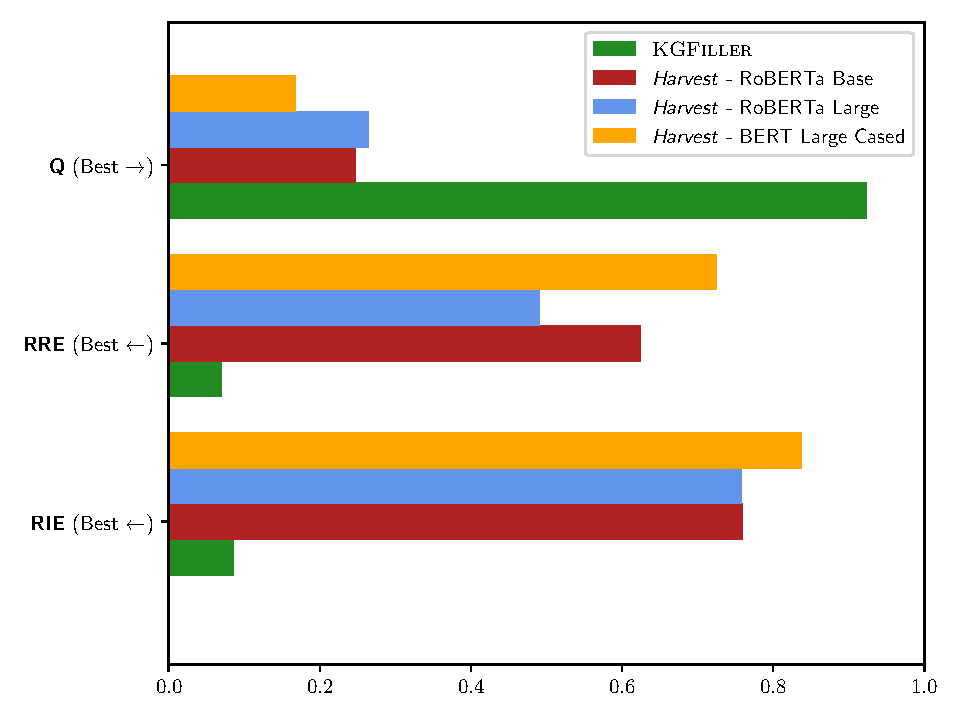
\includegraphics[width=\linewidth]{figures/kgfiller/comparison}
    \caption[Performance Comparison of Harvest and \llmfkg{}]{
        Performance comparison of Harvest~\cite{HaoTTNSZXH23} and \llmfkg{} for populating the food ontology (\Cref{subsubsec:kgfiller-ontology}).
        %
        The best-performing closed-source and open-source \gls{LLM} models are considered: GPT 3.5 Turbo and Nous Hermes, respectively.
    }
    \label{fig:compare-performance}
\end{figure}



\subsection{Discussion and \gls{SWOT} Analysis}
\label{subsec:discussion}

To the best of our knowledge, this work introduces a novel methodology for ontology population, enabling the generation of structured knowledge tailored to specific domains or schemas.
%
This section provides a \gls{SWOT} analysis, highlighting the \textit{Strengths}, \textit{Weaknesses}, \textit{Opportunities}, and \textit{Threats} of \llmfkg{}.
%
The discussion transitions from technical aspects to strategic considerations, including potential applications, limitations, and future directions.

\subsubsection{Strengths}
\label{subsubsec:strengths}

\paragraph{Automation}
%
\llmfkg{} leverages \glspl{LLM} trained on extensive general-knowledge datasets.
%
This eliminates the need for large \emph{corpora} of textual documents and makes it the first fully automatic ontology population method.
%
No prior domain knowledge representation is required from the user.

\paragraph{Generality}
%
\glspl{LLM} enable \llmfkg{} to operate across virtually any domain, irrespective of the availability of domain-specific data.
%
Unlike traditional methods, which rely on potentially incomplete or biased document collections, \llmfkg{} benefits from the broad and diverse knowledge embedded in \glspl{LLM}.

\paragraph{Incrementality}
%
\llmfkg{} supports both ontology population and refinement.
%
It can be applied iteratively to enrich existing ontologies, allowing for incremental improvements over multiple runs.
%
This flexibility contrasts with traditional methods, which are often constrained by predefined input datasets.

\paragraph{Future Potential}

As \glspl{LLM} continue to evolve, their emergent capabilities are expected to enhance the quality of ontology population.
%
Future advancements may enable \llmfkg{} to extract knowledge beyond the explicit content of training data.

\subsubsection{Weaknesses}
\label{subsubsec:weaknesses}
%
\paragraph{Completeness}
%
\llmfkg{} does not guarantee completeness in the populated ontology.
%
Instances or relations may be missing, as the method is not designed to extract all knowledge from the \gls{LLM}.
%
This limitation is inherent to any (semi-)automatic data-driven approach.

\paragraph{Sampling Bias}
%
The reliance on \glspl{LLM} trained on web data introduces potential sampling biases.
%
Underrepresented topics on the web may result in unbalanced or biased ontologies.
%
Further research is needed to mitigate these biases in \glspl{LLM}.

\paragraph{Correctness}
%
\llmfkg{} cannot ensure the correctness of extracted information.
%
\glspl{LLM} are prone to hallucinations, which may lead to the inclusion of false or misleading data in the ontology~\cite{hallucination-2023}.
%
Careful validation of the populated ontology is necessary to address this limitation.


\subsubsection{Opportunities}
\label{subsubsec:opportunities}
%
\paragraph{Cold Start}
%
\llmfkg{} addresses the cold start problem in knowledge-based systems by providing a quick and cost-effective way to generate domain-specific data.
%
This capability is particularly valuable in early-stage projects where data availability is limited.

\paragraph{Automatic Hierarchy Construction}
%
Extensions of \llmfkg{} could enable the automatic construction of ontology schemas, a task often referred to as \emph{hierarchy construction}~\cite{funk2023ontology}.
%
Such advancements could automate the entire ontology creation process, combining schema construction with population.


\paragraph{Zero-Shot Ontology Creation}
%
Building on the idea of hierarchy construction, \llmfkg{} could be adapted to create ontologies from scratch.
%
This would involve generating both the schema and instances based on a natural-language description of the domain.

\paragraph{Procedural Knowledge Extraction}
%
\llmfkg{} could be extended to extract procedural knowledge, representing structured steps to achieve specific goals.
%
This application has potential in fields like automated planning and \glspl{MAS}, where agents require executable plans to perform tasks.


\subsubsection{Threats}
\label{subsubsec:threats}
%
\paragraph{Dependence on \glspl{LLM}}
%
The effectiveness of \llmfkg{} is tied to the quality and capabilities of the underlying \glspl{LLM}.
%
Limitations in \glspl{LLM}, such as biases or inaccuracies, directly impact the quality of the populated ontology.

\paragraph{Cost and Efficiency}
%
The computational and financial costs of querying \glspl{LLM} may pose challenges, especially for large-scale ontology population tasks.
%
Optimizing the process to balance cost and quality remains an open research question.

\paragraph{Ethical Concerns}
%
The use of \glspl{LLM} trained on web data raises ethical concerns, including data privacy and the propagation of biases.
%
Addressing these issues is critical to ensure responsible deployment of \llmfkg{}.

% The SWOT analysis highlights the potential and limitations of \llmfkg{},
% providing a roadmap for future research and development.


\subsection{Conclusion}
\label{subsec:kgfiller-conclusion}
%
Ontologies provide a structured framework to define concepts, relationships, and properties within a specific domain.
%
This ensures an unambiguous and comprehensible representation of domain-specific knowledge.
%
However, the process of ontology population is often meticulous, time-consuming, and prone to human errors and biases.
%

In this work, we hypothesize that \glspl{LLM}\footnote{Defined in \texttt{my\_acronyms.sty}} embed a significant amount of domain-specific knowledge.
%
This knowledge is acquired during their domain-agnostic training on vast datasets collected from the Web.
%
Based on this hypothesis, we propose \llmfkg{}, a novel approach for automatic ontology population leveraging \glspl{LLM}.
%

The proposed method starts with:
%
\begin{inlinelist}
    \item an initial schema consisting of interrelated classes and properties, and
    %
    \item a set of query templates.
\end{inlinelist}
%
\llmfkg{} queries the \gls{LLM} multiple times to generate instances for classes, relationships, and properties based on its responses.
%
Additional queries are performed to refine the ontology, ensuring balanced class hierarchies and avoiding duplicate entries.
%

The validity of \llmfkg{} is demonstrated through a case study in the food domain.
%
This domain requires the population of an ontology with food ingredients, categorized across multiple classes, and recipes.
%
We evaluate \llmfkg{} using various state-of-the-art \glspl{LLM}, including open-source, closed-source, and \glspl{MoE}.
%
The evaluation employs a range of metrics to assess the quality of the constructed ontology.
%

Our results show that \llmfkg{} reliably populates ontologies across different \glspl{LLM}.
%
For instance, the GPT 3.5 model achieves accuracies of up to \(0.91\) for instances and \(0.93\) for relations.
%
As expected, larger \glspl{LLM} generally perform better.
%
We also observe a correlation between erroneous instances and misplaced relations, highlighting areas for improvement.
%

Finally, we analyze the severity of errors, emphasizing how hallucinations from \glspl{LLM} can negatively impact the ontology population process.
%
Despite these challenges, the results are promising.
%
They demonstrate that the complex task of ontology construction can be partially automated, requiring only minor post-processing efforts.
%



\section{Actively learning \EL terminologies from \glspl{LLM}}\label{sec:actively-learning-ontologies}
%
We now present the paper ``Actively Learning \EL Terminologies from Large Language Models'', accepted at the 28th European Conference on Artificial Intelligence (ECAI 2025)\footnote{\url{https://ecai2025.org/}}.
%
In active learning, a \emph{learner} attempts to learn from a \emph{teacher} by posing questions.
%
The questions made by the learner are called \emph{membership queries} and are answered with `yes' or `no'.
%
This kind of query is often studied as part of a communication protocol that also includes \emph{equivalence queries}.
%
Intuitively, equivalence queries ask whether the idea of the learner about the knowledge of the teacher is correct or not.
%
If not, then the teacher should provide a counterexample showing the difference (or equivalently, with `true' or `false').
%
In this work, we consider the teacher as a \gls{LLM} and study the case in which knowledge is expressed as an \EL terminology.
%
Membership queries ask whether concept inclusions are true or not.
%
Equivalence queries are simulated by a sample with concept inclusions labelled as  positive or negative.
%
We present a non-trivial extension of the ExactLearner tool to extract \EL terminologies from \glspl{LLM}.
%
The ExactLearner was originally designed to run with a synthetic teacher that answers membership queries together with equivalence queries.
%
Given the relevant symbols as input (e.g., algae, plant, etc.), the tool tries to find how these symbols should be logically connected by posing questions to \glspl{LLM}.
%
To evaluate the approach, we present performance results of the ExactLearner in the task of reconstructing existing \EL terminologies.


\subsection{Introduction}
\label{subsec:actively-learning-introduction}
\glspl{LLM} have accumulated vast amounts of information and significantly improved their question-answering capabilities.
%
This has led to the development of methods to interact with and extract knowledge from these models.
%
Prompts to \glspl{LLM} range from general knowledge questions, such as definitions and historical events, to domain-specific queries, such as scientific facts in health and medicine.
%
Recent efforts have focused on automating the extraction of knowledge from \glspl{LLM}, often representing this knowledge in the form of an \emph{ontology}~\cite{10.1093/bioinformatics/btae104,DBLP:journals/kbs/CiattoAMO25,DBLP:conf/ekaw/DurantiGMRR24,funk2023ontology,DBLP:conf/ontobras/SoaresW24}.
%
Ontologies, a cornerstone of \gls{KR}, provide a structured representation of the conceptual knowledge within a domain.
%
The most widely used formalism for specifying ontologies is \emph{description logic}~\cite{DBLP:books/daglib/0041477}.
%
In life sciences, ontologies are extensively used for tasks such as data integration, information retrieval, and automated reasoning~\cite{DBLP:conf/semweb/NoySDDGJMRYM08}.

%
A key question arises: \emph{What can we learn from \glspl{LLM}?}
%
Moreover, given that \glspl{LLM} can produce incorrect or inconsistent information, is there an automated way to identify such inaccuracies?
%
To address these questions, this work explores an active learning approach to construct \emph{description logic ontologies} from \glspl{LLM}.
%
Our approach is grounded in Angluin's exact learning framework~\cite{DBLP:journals/ml/Angluin87}, where a \emph{learner} acquires knowledge from a \emph{teacher} by posing queries.
%
This method, known as \emph{active learning}~\cite{DBLP:conf/stoc/Angluin92}, involves two types of queries: \emph{membership queries} and \emph{equivalence queries}.
%
Here, we consider the \gls{LLM} as the teacher and aim to learn ontologies formulated in the \EL description logic~\cite{DBLP:conf/ijcai/BaaderBL05}.

%
Exact learning of lightweight description logic ontologies has been studied extensively for theoretical purposes~\cite{DBLP:conf/ijcai/FunkJLPW19,DBLP:conf/ijcai/FunkJL21,DBLP:conf/aaai/KonevOW16,DBLP:journals/jmlr/KonevLOW17,DBLP:conf/dlog/OzakiPM20}.
%
However, a major challenge in applying these algorithms is finding a suitable teacher capable of answering the required queries.
%
The only known implementation for exact learning of \EL ontologies is the \emph{ExactLearner} tool~\cite{DBLP:conf/kr/DuarteKO18}.
%
This tool learns \EL terminologies\footnote{An \EL terminology is an ontology with specific syntactic restrictions (see~\Cref{subsec:active-learning-ontologies})} from a synthetic teacher that can answer membership and equivalence queries.
%
Membership queries verify whether a given concept inclusion is true or false, while equivalence queries check whether the learner's hypothesis matches the teacher's knowledge.
%
If the hypothesis is incorrect, the teacher provides a counterexample.

%
The synthetic teacher in \emph{ExactLearner} was designed to test the tool using ontologies from the Oxford Ontology Repository\footnote{\url{https://www.cs.ox.ac.uk/isg/ontologies/}}.
%
Given a set of relevant symbols, referred to as the \emph{vocabulary} or \emph{signature} (e.g., algae, plant), the tool determines how these symbols are logically connected by posing queries to the teacher.

%
In this work, we extend the \emph{ExactLearner} tool to interact with \glspl{LLM} as teachers, naming the extended version \emph{ExactLearner+LLM}.
%
We use the Manchester OWL Syntax~\cite{DBLP:conf/owled/HorridgeDGRSW06} and a custom parsing function to translate concept inclusions from description logic into natural language.
%
While membership queries can be directly mapped to a question-answering setting with \glspl{LLM}, equivalence queries are more challenging~\cite{DBLP:journals/ml/WeissGY24,BLUM2023109026}.
%
To address this, we simulate equivalence queries using a sample of randomly generated concept inclusions classified as true or false by the \gls{LLM}.
%
This approach aligns with the theoretical analysis of Angluin's framework within the \gls{PAC} learning paradigm~\cite{DBLP:journals/ml/Angluin87}.

%
To evaluate our approach, we conducted experiments using \emph{ExactLearner+LLM} with open-source \glspl{LLM}.
%
The tool was provided with a signature and tasked with reconstructing existing ontologies.
%
We tested it on small ontologies from the original \emph{ExactLearner} benchmark and modules extracted from the GALEN ontology~\cite{Rector2008TheGH}, which contains medical terms.
%
Our results also examine whether there is statistical evidence of correlation between the concept inclusions extracted by \emph{ExactLearner+LLM} and those in the original ontologies created by human engineers.
%
% This highlights the potential of \glspl{LLM} in ontology construction.


\subsection{Background and related work}
\label{subsec:active-learning-ontologies}
%
In this section, we define the concept of an \EL terminology, elaborate on the exact and \gls{PAC} learning frameworks, and describe the algorithm implemented in the \emph{ExactLearner} tool~\cite{DBLP:conf/kr/DuarteKO18}, which is designed to learn \EL terminologies from a teacher capable of answering membership and equivalence queries.
%
\paragraph{The \EL Description Logic}
Let \(\NC\) and \(\NR\) be countably infinite and disjoint sets of \emph{concept names} and \emph{role names}, respectively.
%
In some cases, we may consider \(\NC\) and \(\NR\) as finite sets, depending on the context.
%
An \EL \emph{concept} is defined as \(C, D \coloneqq C \sqcap D \mid \exists r.C \mid A \mid \top\), where \(A \in \NC\) and \(r \in \NR\).
%
An \EL \emph{concept inclusion} is an expression of the form \(C \sqsubseteq D\), where \(C\) and \(D\) are \EL concepts.
%
An \EL \emph{equivalence} is expressed as \(C \equiv D\), which is equivalent to \(C \sqsubseteq D\) and \(D \sqsubseteq C\).
%
An \EL \emph{ontology} is a finite set of \EL concept inclusions \(C \sqsubseteq D\).
%
For a given ontology \(\Omc\), we denote the sets of concept names and role names occurring in \(\Omc\) as \(\NC(\Omc)\) and \(\NR(\Omc)\), respectively.
%
These sets are also referred to as the \emph{signature} of \(\Omc\).
%
If, for all concept inclusions \(C \sqsubseteq D\) in \(\Omc\), at least one of \(C\) or \(D\) belongs to \(\NC\), and there is at most one inclusion of the form \(A \sqsubseteq C\) for every \(A \in \NC\), then \(\Omc\) is called a \emph{terminology}\footnote{This definition is slightly more flexible than the standard one in the description logic literature~\cite{DBLP:books/daglib/0041477}.}.
%
The semantics of \EL is defined using interpretations, as described in~\cite{DBLP:books/daglib/0041477}.
%
Given an ontology \(\Omc\) and a concept inclusion \(C \sqsubseteq D\), we say that \(\Omc\) \emph{entails} \(C \sqsubseteq D\), denoted as \(\Omc \models C \sqsubseteq D\), if every interpretation satisfying \(\Omc\) also satisfies \(C \sqsubseteq D\).
%
Two ontologies \(\Omc\) and \(\Hmc\) are \emph{equivalent}, denoted as \(\Omc \equiv \Hmc\), if they are satisfied by the same interpretations.
%
This means that, for all concept inclusions \(C \sqsubseteq D\), \(\Omc \models C \sqsubseteq D \iff \Hmc \models C \sqsubseteq D\).


\paragraph{Exact Learning}
The exact learning framework, introduced by Angluin~\cite{DBLP:journals/ml/Angluin87}, involves a \emph{learner} attempting to acquire a target concept, which in this work is an \EL terminology, from a \emph{teacher}.
%
The communication protocol between the learner and the teacher includes two types of queries:
%
\begin{itemize}
    \item \emph{Membership queries}, where the learner asks whether a specific statement is true or false.
    %
    \item \emph{Equivalence queries}, where the learner proposes a hypothesis and receives either confirmation that the hypothesis matches the target or a counterexample highlighting the difference~\cite{DBLP:journals/ml/Angluin87}.
\end{itemize}
%
In our context, membership queries verify whether an \EL concept inclusion \(C \sqsubseteq D\) is true or false.
%
For example, the learner may ask whether \(\mathsf{Algae} \sqsubseteq \mathsf{Plant}\) holds true.


\paragraph{Simulating Equivalence Queries}
To simulate equivalence queries, we adopt a \emph{sampling} strategy.
%
Instead of directly asking the \gls{LLM} to evaluate the hypothesis and provide a counterexample, we generate a random set of \EL concept inclusions and query the \gls{LLM} to classify them as true or false.
%
We then verify whether the learner's hypothesis is consistent with the \gls{LLM}'s classification.
%
Consistency is achieved if all true concept inclusions are logical consequences of the hypothesis and all false inclusions are not.
%
If the hypothesis is consistent, the learning process terminates.
%
Otherwise, a counterexample is identified, and the process continues as if the \gls{LLM} had returned a counterexample in response to an equivalence query.
%
This approach has been used in prior work to simulate equivalence queries~\cite{DBLP:journals/ml/WeissGY24,BLUM2023109026}.
%
Under certain conditions, this strategy provides theoretical guarantees within the \gls{PAC} learning framework~\cite{DBLP:journals/ml/Angluin87,DBLP:journals/cacm/Valiant84}.
%
In \gls{PAC} learning, the required sample size is determined by the hypothesis space \(\mathbf{H}\) (in this case, \EL terminologies of a specific size and structure defined by a given signature) and two parameters, \(\epsilon\) and \(\delta\), representing the error tolerance and confidence level, respectively.
%
According to \gls{PAC} theory~\cite[Cor. 2.3]{DBLP:books/daglib/0033642}, the sample size must be at least \(\mathsf{\ln}(|\mathbf{H}|/\delta)/\epsilon\) for finite \(\mathbf{H}\).


\paragraph{The Algorithm for \EL Terminologies}
%
\begin{algorithm}
\caption{The learning algorithm for $\mathcal{EL}$~\cite{DBLP:conf/kr/DuarteKO18}}
\label{alg:learn}
\begin{algorithmic}[1]
\State \textbf{Input:} $\NC(\Omc) \cup \NR(\Omc)$ and access to a teacher that can answer membership and equivalence queries (or just membership queries if equivalence queries are simulated in a PAC setting).
\State \textbf{Output:} An $\mathcal{EL}$ terminology $\Hmc$ such that $\Omc \equiv \Hmc$.
\Statex
\State Initialize $\Hmc \gets \{A \sqsubseteq B \mid \Omc \models A \sqsubseteq B, A,B\in \NC(\Omc)\}$
\While{$\Hmc \not\equiv \Omc$} \label{line:while}
    \State Let $C \sqsubseteq D$ be a positive counterexample for $\Omc$ relative to $\Hmc$
    \State Compute $C' \sqsubseteq D'$ with $C'$ or $D'$ in $\NC(\Omc)$
    \label{line:counterexample}
    \If{$C' \in \NC(\Omc)$}
        \State Compute a right $\Omc$-essential $\alpha$ from
        \[
        C' \sqsubseteq D' \sqcap \bigsqcap_{C' \sqsubseteq F' \in \Hmc} F'
        \]
        \label{line:right-essential}
    \Else
        \State Compute a left $\Omc$-essential $\alpha$ from $C' \sqsubseteq D'$
        \label{line:left-essential}
    \EndIf
    \State Add $\alpha$ to $\Hmc$
    \label{line:add-to-hypothesis}
\EndWhile
\State \Return $\Hmc$
\end{algorithmic}
\end{algorithm}
%
The \emph{ExactLearner} tool~\cite{DBLP:conf/kr/DuarteKO18} is designed to learn \EL terminologies by interacting with a synthetic teacher that answers membership and equivalence queries.
%
The teacher's responses are logically consistent with a target \EL terminology, and the communication is conducted in \gls{OWL} rather than natural language.
%
The main steps of the learning procedure are outlined in \Cref{alg:learn}.
%
The algorithm performs equivalence queries in line~\ref{line:while} and membership queries in lines~\ref{line:counterexample},~\ref{line:right-essential}, and~\ref{line:left-essential}.
%
In line~\ref{line:counterexample}, a counterexample \(C' \sqsubseteq D'\) is extracted from \(C \sqsubseteq D\), ensuring that one of the sides belongs to \(\NC(\Omc)\).
%
This step is guaranteed to find a counterexample because \(\Omc\) is a terminology~\cite{DBLP:conf/kr/DuarteKO18}.
%
The algorithm applies various operations using membership queries, including \emph{concept saturation for \(\Omc\)}, \emph{sibling merging}, \emph{decomposition on the right}, and \emph{decomposition on the left}.
%
Additionally, two heuristics, \emph{desaturation} and \emph{branching}, are employed.
%
These operations aim to maximize the informativeness of concept inclusions while minimizing their size.
%
The resulting concept inclusions, referred to as \(\Omc\)-essential, are added to the hypothesis in line~\ref{line:add-to-hypothesis}.


\subsection{\glspl{LLM} as teachers}
\label{subsec:probing}
%
\glspl{LLM} present significant opportunities for acquiring knowledge in the form of ontologies.
%
However, several challenges must be addressed to effectively employ them as teachers in an active learning framework.
%
The main challenges are as follows:
%
\begin{itemize}
    \item Membership queries in the \emph{ExactLearner} tool are expressed in \gls{OWL}, whereas \glspl{LLM} are designed to process natural language inputs.
    %
    \item Responses from \glspl{LLM} may deviate from the expected format, even when explicitly instructed to answer with `yes' or `no'.
    %
    \item Queries generated by the \emph{ExactLearner} can be lengthy and complex, involving multiple logical operators, which may hinder the ability of \glspl{LLM} to provide accurate answers.
    %
    \item Even when responses are concise and well-formatted, they may be logically inconsistent with previous answers or incorrect, and they may vary if the same query is repeated.
    %
    \item The expressivity of the ontology language used (\EL) limits the scope of the knowledge that can be extracted.
\end{itemize}
%
Below, we discuss how these challenges are addressed.


\paragraph{Input Format}
\label{par:input-format}
%
The format of the queries plays a crucial role in ensuring effective communication with \glspl{LLM}.
%
We use both the Manchester \gls{OWL} syntax~\cite{DBLP:conf/owled/HorridgeDGRSW06} and controlled natural language to standardize the queries.
%
Queries in Manchester \gls{OWL} syntax take the form \texttt{[A] SubClassOf [B]}.
%
In natural language, these are translated into questions such as:
%
\begin{center}
    ``Can \texttt{[A]} be considered a subcategory of \texttt{[B]}? Answer only with yes or no.''
\end{center}
%
Here, \texttt{[A]} and \texttt{[B]} are placeholders for the left-hand and right-hand sides of the concept inclusion.
%
This approach aligns with the third formulation proposed by Funk et al.~\cite{funk2023ontology}, which is well-suited to our setting.
%
The translation of \gls{OWL} concept expressions into natural language is applied recursively:
%
\begin{enumerate}
    \item Expressions of the form \texttt{[A] and [B]} are replaced with ``\texttt{[A]} that is also \texttt{[B]}''.
    %
    \item Expressions of the form \texttt{[r] some [A]}, where \texttt{[r]} is a role name, are replaced with ``something that \texttt{[r]} \texttt{[A]}''.
\end{enumerate}
%
\begin{example}\upshape
    The concept inclusion \texttt{Person SubClassOf Human} is translated into:
    %
    ``Can Person be considered a subcategory of Human?''
    %
    Similarly, \texttt{Carnivore SubClassOf Animal and eats some Meat} becomes:
    %
    ``Can Carnivore be considered a subcategory of Animal that is also something that eats Meat?''
    %
    Finally, \texttt{(Bird and Fish) SubClassOf Animal} is translated to:
    %
    ``Can Bird that is also Fish be considered a subcategory of Animal?''
\end{example}


\paragraph{Unexpected Responses}
\label{par:unexpected-responses}
%
\glspl{LLM} may return arbitrary responses, even when the expected answer is a single word such as `true' or `false'.
%
To mitigate this, we explicitly instruct the \gls{LLM} to answer with `true' or `false' by appending this requirement to the query.
%
Alternatively, we use system prompts or adjust hyperparameters, such as temperature, to guide the model's responses.
%
Despite these precautions, unexpected responses may still occur:
%
\begin{enumerate}
    \item The response may include additional text beyond `true' or `false'.
    %
    \item Both `true' and `false' may appear in the response.
    %
    \item Neither `true' nor `false' may be present in the response.
\end{enumerate}
%
To address these issues, we limit the maximum number of tokens in the response.
%
If the response does not contain `true' or `false', we treat it as `false'.


\paragraph{Length of Queries}
\label{par:length-of-queries}
%
Long and complex queries can lead to biased responses from \glspl{LLM}, such as always answering `true'.
%
To address this, we modify the \emph{ExactLearner} tool as follows:
%
\begin{itemize}
    \item \emph{Simplification:} Concept expressions are simplified by removing redundant concept names.
    %
    For example, if $A \sqcap B$ is a concept expression and $A \sqsubseteq B$ is entailed by the hypothesis, $B$ is omitted.
    %
    \item \emph{Splitting:} Long queries with multiple conjuncts are split into smaller queries.
    %
    For instance, instead of asking whether $C \sqsubseteq D_1 \sqcap \ldots \sqcap D_n$, we ask whether $C \sqsubseteq D_1$, $C \sqsubseteq D_2$, and so on.
\end{itemize}
%
These modifications reduce the likelihood of biased responses and improve the accuracy of the \gls{LLM}.


\paragraph{Correctness and Logical Consistency}
\label{par:correctness-and-consistency}
%
Responses from \glspl{LLM} may not always reflect the truth or be logically consistent with an \EL ontology.
%
Errors can occur in the following cases:
%
\begin{enumerate}
    \item A false inclusion $C \sqsubseteq D$ is incorrectly answered as `true'.
    %
    \item A true inclusion $C \sqsubseteq D$ is incorrectly answered as `false'.
    %
    \item The \gls{LLM} answers `true' for all inclusions in an ontology $\Omc$, but answers `false' for a logical consequence of $\Omc$.
\end{enumerate}
%
To handle logical inconsistencies, we compute the \emph{closure} under logical consequence~\cite{BLUM2023109026}.
%
Additionally, we use a caching mechanism to store the first response to each query, ensuring consistency across repeated queries.

%
\paragraph{Expressivity}
\label{par:expressivity}
%
The algorithm focuses on extracting \EL terminologies, which may not fully capture knowledge better expressed in more expressive languages.
%
However, \EL is widely used in real-world ontologies, particularly in the medical domain~\cite{Rector2008TheGH,bioportal}.
%
Its polynomial-time reasoning complexity~\cite{DBLP:conf/ijcai/BaaderBL05} and the availability of efficient reasoning tools~\cite{DBLP:journals/jar/KazakovKS14} make it a practical choice for ontology construction.



\subsection{Experiments}
\label{subsec:experiments}

The code for the experiments is publicly available on GitHub\footnote{\url{https://github.com/MatteoMagnini/ExactLearner-LLM/}}.
%
All experiments were conducted on a workstation equipped with two NVIDIA Tesla V100S-PCIE-32GB GPUs and dual Intel\textcopyright~Xeon\textcopyright~Gold 6226R CPUs, providing a total of 64 threads.
%
The system was configured with CUDA 12.5 and NVIDIA driver version 535.183.01.
%

\paragraph{Evaluation Approach}
\label{par:evaluation-approach}
\Cref{alg:learn} takes as input the signature, which consists of finite sets of concept and role names, and constructs an \gls{EL} terminology by posing membership and equivalence queries.
%
Equivalence queries are simulated using a \emph{\gls{PAC} sample}, which is a set of concept inclusions randomly generated and answered by the \gls{LLM}.
%
For an ontology \(\Omc\) with \(n\) logical axioms, the \gls{PAC} sample size is computed as:
\[
\frac{\ln(A^n / \delta)}{\epsilon},
\]
where \(\delta = 0.1\), \(\epsilon = 0.2\), and \(A\) is the number of all possible axioms of the form:
\[
A \sqsubseteq B, \quad A \sqcap B \sqsubseteq C, \quad B \sqsubseteq \exists r.A, \quad \text{and} \quad \exists r.A \sqsubseteq B,
\]
with \(A, B, C \in \NC\) and \(r \in \NR\), formulated using the signature of \(\Omc\).
%
We refer to these axioms as \emph{normalized}.
%
The ability of ExactLearner+LLM to reconstruct existing ontologies is tested by posing queries to the \gls{LLM}.
%

\paragraph{Hypotheses}
\label{par:hypotheses}
We test the following hypotheses in our experiments:
%
\begin{enumerate}
    \item Even though \glspl{LLM} may make mistakes and the simulation strategy does not guarantee exact learnability, we expect a correlation between the ontologies built by ExactLearner+LLM and the original ontologies.
    %
    \item Queries expressed in controlled natural language using our parsing function will yield better results than those using the OWL Manchester syntax.
    %
    \item Larger \glspl{LLM} will perform better than smaller ones.
    %
    \item Ontologies expressing common knowledge, such as family relations, will be easier to learn than those with specialized knowledge, such as medical ontologies.
    %
    \item Simplifications introduced to reduce query length (see \Cref{subsec:probing}) will improve the performance of \glspl{LLM} and, consequently, the ontologies constructed by ExactLearner+LLM.
\end{enumerate}
%

\paragraph{Datasets}
\label{par:datasets}
We use two datasets:
%
\begin{enumerate}
    \item Five small ontologies from the ExactLearner benchmark~\cite{DBLP:conf/kr/DuarteKO18}.
    %
    \item Ten modules extracted from the GALEN ontology~\cite{Rector2008TheGH}, which contains medical information.
\end{enumerate}
%
The small ontologies include:
%
\begin{itemize}
    \item \emph{Animals}, which describes the animal realm, including subphyla, classes, and orders.
    %
    \item \emph{Cell}, which provides information about cells based on type, development stage, and organism.
    %
    \item \emph{Football}, a minimal ontology describing relations between football games, teams, players, and managers.
    %
    \item \emph{Generations}, which describes family members and their relations.
    %
    \item \emph{University}, focusing on the professor role.
\end{itemize}
%
\Cref{tab:small-ontologies} summarizes the size of the signature, logical axioms, \gls{PAC} sample size, and possible normalized axioms for these ontologies.
\begin{table}[]
\centering
\caption[Small Ontologies Statistics and \gls{PAC} Sample Sizes]{
    Ontology statistics and \glsentryshort{PAC} sample sizes with $\epsilon=0.2$ and $\gamma=0.1$.
    $\NC$ and $\NR$ are the number of concept and role names occurring in the ontologies.
}
\label{tab:small-ontologies}
\resizebox{\columnwidth}{!}{
\begin{tabular}{|l|c|c|c|c|c|}
\hline
\textbf{Ontology} & \textbf{$\NC$} & \textbf{$\NR$} & \textbf{Log. Ax.} & \textbf{PAC Sample} & \textbf{Poss. Ax.} \\
\hline
\rowcolor[HTML]{EFEFEF}
Animals & 17 & 4 & 12 & 542 & 6,936\\
\hline
\rowcolor[HTML]{FFFFFF}
Cell & 22 & 0 & 24 & 1,119 & 10,164\\
\hline
\rowcolor[HTML]{EFEFEF}
Football & 10 & 3 & 9 & 341 & 1,500\\
\hline
\rowcolor[HTML]{FFFFFF}
Generations & 20 & 4 & 18 & 847 & 10,800\\
\hline
\rowcolor[HTML]{EFEFEF}
University & 7 & 3 & 4 & 139 & 588\\
\hline
\end{tabular}}
\end{table}

%

The GALEN ontology is a large medical ontology with \(22,286\) concept names, \(950\) role names, and \(46,558\) logical axioms.
%
Since not all axioms are connected, we modularize GALEN using the bottom locality strategy~\cite{DBLP:journals/jair/GrauHKS08}\footnote{\url{https://github.com/ernestojimenezruiz/locality-module-extractor}}.
%
This method generates \(22,286\) modules, one for each concept name.
%
We randomly select 10 modules, ensuring each has at least one concept and one role name, and no more than 50 concept or role names.
%
\Cref{tab:modules-ontologies} lists the selected modules.
\begin{table}[]
\centering
\caption{Ontology statistics and \gls{PAC} sample sizes with $\epsilon=0.2$ and $\gamma=0.1$ for medical ontologies.}
\label{tab:modules-ontologies}
\resizebox{\columnwidth}{!}{
\begin{tabular}{|l|c|c|c|c|c|}
\hline
\textbf{Ontology} & \textbf{\NC} & \textbf{\NR} & \textbf{Log. Ax.} & \textbf{PAC Sample}  & \textbf{Pos. Ax.}  \\
\hline
\rowcolor[HTML]{EFEFEF}
Ab. Elb. J. C. & 27 & 14 & 43 & 2,286 & 39,366\\
\hline
\rowcolor[HTML]{FFFFFF}
BNF Sec. & 36 & 24 & 80 & 4,646 & 107,568\\
\hline
\rowcolor[HTML]{EFEFEF}
Chlorhexidine & 23 & 14 & 38 & 1,946 & 26,450\\
\hline
\rowcolor[HTML]{FFFFFF}
Cone of Tissue & 42 & 42 & 100 & 6,163 & 220,500\\
\hline
\rowcolor[HTML]{EFEFEF}
Kalli Krein & 18 & 10 & 27 & 1,279 & 11,988\\
\hline
\rowcolor[HTML]{FFFFFF}
Neon & 16 & 10 & 25 & 1,149 & 8,960\\ 
\hline
\rowcolor[HTML]{EFEFEF}
Pin & 43 & 40 & 99 & 6,113 & 225,578\\
\hline
\rowcolor[HTML]{FFFFFF}
Pros. Drug & 29 & 14 & 47 & 2,540 & 47,096\\
\hline
\rowcolor[HTML]{EFEFEF}
Zopiclone & 32 & 36 & 77 & 4,465 & 105,472\\
\hline
\rowcolor[HTML]{FFFFFF}
Zuccini & 33 & 22 & 58 & 3,295 & 82,764\\
\hline
\end{tabular}}
\end{table}

%

\paragraph{LLMs, Query Format, and Prompts}
We use four open \glspl{LLM}: Mistral~\cite{mistral} (7B parameters), Mixtral~\cite{mixtral} (47B parameters), Llama2 (13B parameters), and Llama3 (8B parameters)~\cite{llama2}, accessed via Ollama's API\footnote{\url{https://github.com/ollama/ollama}}.
%
Queries are expressed in either Manchester OWL syntax or controlled natural language (see \Cref{par:input-format}).
%
We use two system prompts:
%
\begin{promptbox}[Simple system prompt]
    \scriptsize
    Answer with only True or False.
\end{promptbox}
%
\begin{promptbox}[Advanced system prompt]
    \scriptsize
    You need to classify the following statements as True or False. The statement will be provided in either Manchester OWL syntax or natural language. Strictly follow these guidelines:

    1. Answer with only True or False.

    2. Entities with \texttt{has part} relations are not in a subclass relation.

    3. Statements containing numerous entities are most probably False.

    4. Take a deep breath before answering.

    5. If unsure, answer False.
\end{promptbox}
%
The advanced prompt provides additional contextual information and guidelines to improve \gls{LLM} performance.
%
For instance, it emphasizes that entities with \texttt{has part} relations should not be in a subclass relation~\cite{funk2023ontology}.
%
It also mitigates the tendency of \glspl{LLM} to answer ``True'' to long queries, which may arise during the computation of \(\Omc\)-essential concept inclusions (\Cref{subsec:active-learning-ontologies}).
%

\paragraph{Experimental Details}
To constrain \gls{LLM} responses, we limit the maximum number of tokens to 2, ensuring answers are either ``True'' or ``False''\footnote{A token is a unit of text, typically corresponding to a few characters. For example, ``False'' requires 2 tokens. See \url{https://help.openai.com/en/articles/4936856}.}.
%
We also employ a caching mechanism to store \gls{LLM} responses, reducing computation time and ensuring consistency when the same query is posed multiple times.



\subsection{Evaluation and Results}
\label{subsec:evaluation-and-results}
%
We evaluate the experimental results by computing the following metrics: accuracy, precision, recall, and F1-score.
%
These metrics are calculated considering all possible axioms of the form:
%
\[
A \sqsubseteq B, \quad A \sqcap B \sqsubseteq C, \quad B \sqsubseteq \exists r.A, \quad \text{and} \quad \exists r.A \sqsubseteq B,
\]
%
where \(A, B, C \in \NC\) and \(r \in \NR\), formulated using a finite signature.
%
Tautologies, such as \(A \sqsubseteq A\), \(A \sqcap B \sqsubseteq B\), and \(A \sqcap B \sqsubseteq A\), are excluded to avoid artificially inflating the number of true positives.
%
Our language does not allow for the expression of contradictions.

%
Axioms entailed by both the original and the learned ontology are labeled as true positives.
%
Those not entailed by either are labeled as true negatives.
%
Axioms entailed by the original ontology but not by the learned one are labeled as false negatives, and vice versa for false positives.

%
\subsubsection{Learning Performance}
\label{subsubsec:learning-performance}
%

\begin{table}[]
\centering
\caption{Results of ExactLearner+LLM grouped by ontologies.}
\label{tab:results-small-ontologies}
\resizebox{\columnwidth}{!}{
\begin{tabular}{|l|c|c|c|c|}
\hline
\textbf{Ontology} & \textbf{Accuracy} & \textbf{Recall} & \textbf{Precision} & \textbf{F1-Score} \\
\hline
\rowcolor[HTML]{EFEFEF}
Animals & 0.737 & 0.858 & 0.381 & 0.428 \\
\hline
\rowcolor[HTML]{FFFFFF}
Cell & 0.391 & 0.733 & 0.206 & 0.284 \\
\hline
\rowcolor[HTML]{EFEFEF}
Football & 0.553 & 0.89 & 0.422 & 0.477 \\
\hline
\rowcolor[HTML]{FFFFFF}
Generations & 0.691 & 0.658 & 0.564 & 0.476 \\
\hline
\rowcolor[HTML]{EFEFEF}
University & 0.622 & 0.629 & 0.313 & 0.302 \\
\hline
\end{tabular}}
\end{table}


\begin{table}[]
\centering
\caption{Results of ExactLearner+LLM grouped by models.}
\label{tb:results-small-models}
\resizebox{\columnwidth}{!}{
\begin{tabular}{|l|c|c|c|c|}
\hline
\textbf{Model} & \textbf{Accuracy} & \textbf{Recall} & \textbf{Precision} & \textbf{F1-Score} \\
\hline
\rowcolor[HTML]{EFEFEF}
Llama2 (13b) & 0.521 & 0.71 & 0.294 & 0.314 \\
\hline
\rowcolor[HTML]{FFFFFF}
Llama3 (8b) & 0.43 & 0.947 & 0.218 & 0.333 \\
\hline
\rowcolor[HTML]{EFEFEF}
Mistral (7b) & 0.741 & 0.747 & 0.45 & 0.49 \\
\hline
\rowcolor[HTML]{FFFFFF}
Mixtral (47b) & 0.705 & 0.611 & 0.547 & 0.436 \\
\hline
\end{tabular}}
\end{table}


\begin{table}[]
\centering
\caption{Results of  ExactLearner+LLM grouped by prompts.}
\label{tb:results-small-prompt}
\resizebox{\columnwidth}{!}{
\begin{tabular}{|l|c|c|c|c|}
\hline
\textbf{Prompt Type} & \textbf{Accuracy} & \textbf{Recall} & \textbf{Precision} & \textbf{F1-Score} \\
\hline
\rowcolor[HTML]{EFEFEF}
M. OWL Syntax & 0.34 & 0.93 & 0.165 & 0.262 \\
\hline
\rowcolor[HTML]{FFFFFF}
Natural Language & 0.751 & 0.811 & 0.414 & 0.511 \\
\hline
\rowcolor[HTML]{EFEFEF}
A. M. OWL Syntax & 0.537 & 0.767 & 0.326 & 0.347 \\
\hline
\rowcolor[HTML]{FFFFFF}
A. Natural Language & 0.767 & 0.506 & 0.603 & 0.454 \\
\hline
\end{tabular}}
\end{table}
%
\begin{table}[ht]
\centering
\caption[Results on the Animals ontology]{
    Individual results of ExactLearner+LLM on the Animals ontology.
    %
    All the results have been analysed with the Chi-Squared test. The null hypothesis is that there is no correlation between the ontology constructed by ExactLearner+LLM and the Animals ontology. They all have p-value lower than 0.05 (i.e., refused null hypothesis).
}
\label{tab:results-animal}
\resizebox{0.48\textwidth}{!}{
\begin{tabular}{|l|l|l|l|l|l|}
\hline
\multicolumn{1}{|c|}{\textbf{Model}} & \multicolumn{1}{|c|}{\textbf{Prompt \& Query}} & \multicolumn{1}{c|}{\textbf{Accuracy}} & \multicolumn{1}{c|}{\textbf{Recall}} & \multicolumn{1}{c|}{\textbf{Precision}} & \multicolumn{1}{c|}{\textbf{F1-Score}} \\
\hline
\multirow{4}{*}{Llama2 (13b)} 
 & \cellcolor[HTML]{EFEFEF} M. OWL Syntax         & \cellcolor[HTML]{EFEFEF} 0.276 & \cellcolor[HTML]{EFEFEF} 0.982 & \cellcolor[HTML]{EFEFEF} 0.074 & \cellcolor[HTML]{EFEFEF} 0.138 \\ \cline{2-6}
 & Natural Language                               & 0.859 & 0.930 & 0.286 & 0.437 \\ \cline{2-6}
 & \cellcolor[HTML]{EFEFEF} E. M. OWL Syntax      & \cellcolor[HTML]{EFEFEF} 0.380 & \cellcolor[HTML]{EFEFEF} 0.945 & \cellcolor[HTML]{EFEFEF} 0.083 & \cellcolor[HTML]{EFEFEF} 0.152 \\ \cline{2-6}
 & E. Natural Language                            & 0.970 & 0.651 & 0.801 & 0.718 \\ \cline{1-6}
\hline
\multirow{4}{*}{Llama3 (8b)} 
 & \cellcolor[HTML]{EFEFEF} M. OWL Syntax         & \cellcolor[HTML]{EFEFEF} 0.309 & \cellcolor[HTML]{EFEFEF} 1.000 & \cellcolor[HTML]{EFEFEF} 0.078 & \cellcolor[HTML]{EFEFEF} 0.145 \\ \cline{2-6}
 & Natural Language                               & 0.920 & 0.890 & 0.414 & 0.565 \\ \cline{2-6}
 & \cellcolor[HTML]{EFEFEF} E. M. OWL Syntax      & \cellcolor[HTML]{EFEFEF} 0.314 & \cellcolor[HTML]{EFEFEF} 0.985 & \cellcolor[HTML]{EFEFEF} 0.078 & \cellcolor[HTML]{EFEFEF} 0.145 \\ \cline{2-6}
 & E. Natural Language                            & 0.894 & 0.842 & 0.339 & 0.483 \\ \cline{1-6}
\hline
\multirow{4}{*}{Mistral (7b)} 
 & \cellcolor[HTML]{EFEFEF} M. OWL Syntax         & \cellcolor[HTML]{EFEFEF} 0.552 & \cellcolor[HTML]{EFEFEF} 0.996 & \cellcolor[HTML]{EFEFEF} 0.116 & \cellcolor[HTML]{EFEFEF} 0.207 \\ \cline{2-6}
 & Natural Language                               & 0.955 & 0.912 & 0.575 & 0.706 \\ \cline{2-6}
 & \cellcolor[HTML]{EFEFEF} E. M. OWL Syntax      & \cellcolor[HTML]{EFEFEF} 0.830 & \cellcolor[HTML]{EFEFEF} 0.945 & \cellcolor[HTML]{EFEFEF} 0.250 & \cellcolor[HTML]{EFEFEF} 0.396 \\ \cline{2-6}
 & E. Natural Language                            & 0.943 & 0.890 & 0.511 & 0.649 \\ \cline{1-6}
\hline
\multirow{4}{*}{Mixtral (47b)} 
 & \cellcolor[HTML]{EFEFEF} M. OWL Syntax         & \cellcolor[HTML]{EFEFEF} 0.712 & \cellcolor[HTML]{EFEFEF} 0.904 & \cellcolor[HTML]{EFEFEF} 0.158 & \cellcolor[HTML]{EFEFEF} 0.269 \\ \cline{2-6}
 & Natural Language                               & 0.970 & 0.893 & 0.690 & 0.779 \\ \cline{2-6}
 & \cellcolor[HTML]{EFEFEF} E. M. OWL Syntax      & \cellcolor[HTML]{EFEFEF} 0.960 & \cellcolor[HTML]{EFEFEF} 0.739 & \cellcolor[HTML]{EFEFEF} 0.636 & \cellcolor[HTML]{EFEFEF} 0.684 \\ \cline{2-6}
 & E. Natural Language                            & 0.955 & 0.228 & 1.000 & 0.371 \\ \cline{1-6}
\hline
\end{tabular}
}
\end{table}


%
\begin{table}[ht]
\centering
\caption[Results on the Cell ontology]{
    Individual results of ExactLearner+LLM on the Cell ontology.
    %
    All the results have been analysed with the Chi-Squared test.
    %
    The null hypothesis is that there is no correlation between the ontology constructed by ExactLearner+LLM and the Cell ontology.
    %
    A yellow line means that the p-value is greater than 0.05 (i.e., the null hypothesis cannot be refused).
    %
    The red line means that no axiom has been learnt (i.e., empty ontology).
}
\label{tab:results-cell}
\resizebox{0.48\textwidth}{!}{
\begin{tabular}{|l|l|l|l|l|l|}
\hline
\multicolumn{1}{|c|}{\textbf{Model}} & \multicolumn{1}{|c|}{\textbf{Prompt \& Query}} & \multicolumn{1}{c|}{\textbf{Accuracy}} & \multicolumn{1}{c|}{\textbf{Recall}} & \multicolumn{1}{c|}{\textbf{Precision}} & \multicolumn{1}{c|}{\textbf{F1-Score}} \\
\hline
\multirow{4}{*}{Llama2 (13b)}
 & \cellcolor[HTML]{FFFF00} M. OWL Syntax       & \cellcolor[HTML]{FFFF00} 0.163 & \cellcolor[HTML]{FFFF00} 1.0 & \cellcolor[HTML]{FFFF00} 0.163 & \cellcolor[HTML]{FFFF00} 0.280 \\ \cline{2-6}
 & Natural Language                               & 0.586 & 0.715 & 0.241 & 0.360 \\ \cline{2-6}
 & \cellcolor[HTML]{FFFF00} E. M. OWL Syntax    & \cellcolor[HTML]{FFFF00} 0.163 & \cellcolor[HTML]{FFFF00} 1.0 & \cellcolor[HTML]{FFFF00} 0.163 & \cellcolor[HTML]{FFFF00} 0.280 \\ \cline{2-6}
 & E. Natural Language                            & 0.830 & 0.002 & 0.049 & 0.005 \\ \cline{1-6}
\hline
\multirow{4}{*}{Llama3 (8b)}
 & \cellcolor[HTML]{FFFF00} M. OWL Syntax       & \cellcolor[HTML]{FFFF00} 0.163 & \cellcolor[HTML]{FFFF00} 1.0 & \cellcolor[HTML]{FFFF00} 0.163 & \cellcolor[HTML]{FFFF00} 0.280 \\ \cline{2-6}
 & Natural Language                               & 0.208 & 1.0 & 0.171 & 0.292 \\ \cline{2-6}
 & \cellcolor[HTML]{EFEFEF} E. M. OWL Syntax    & \cellcolor[HTML]{EFEFEF} 0.208 & \cellcolor[HTML]{EFEFEF} 1.0 & \cellcolor[HTML]{EFEFEF} 0.171 & \cellcolor[HTML]{EFEFEF} 0.292 \\ \cline{2-6}
 & E. Natural Language                            & 0.254 & 1.0 & 0.179 & 0.304 \\ \cline{1-6}
\hline
\multirow{4}{*}{Mistral (7b)}
 & \cellcolor[HTML]{EFEFEF} M. OWL Syntax       & \cellcolor[HTML]{EFEFEF} 0.254 & \cellcolor[HTML]{EFEFEF} 1.0 & \cellcolor[HTML]{EFEFEF} 0.179 & \cellcolor[HTML]{EFEFEF} 0.304 \\ \cline{2-6}
 & Natural Language                               & 0.779 & 0.432 & 0.354 & 0.390 \\ \cline{2-6}
 & \cellcolor[HTML]{EFEFEF} E. M. OWL Syntax    & \cellcolor[HTML]{EFEFEF} 0.224 & \cellcolor[HTML]{EFEFEF} 0.946 & \cellcolor[HTML]{EFEFEF} 0.167 & \cellcolor[HTML]{EFEFEF} 0.284 \\ \cline{2-6}
 & E. Natural Language                            & 0.769 & 0.337 & 0.308 & 0.322 \\ \cline{1-6}
\hline
\multirow{4}{*}{Mixtral (47b)}
 & \cellcolor[HTML]{FFFF00} M. OWL Syntax       & \cellcolor[HTML]{FFFF00} 0.163 & \cellcolor[HTML]{FFFF00} 1.0 & \cellcolor[HTML]{FFFF00} 0.163 & \cellcolor[HTML]{FFFF00} 0.280 \\ \cline{2-6}
 & Natural Language                               & 0.654 & 0.970 & 0.317 & 0.477 \\ \cline{2-6}
 & \cellcolor[HTML]{EFEFEF} E. M. OWL Syntax    & \cellcolor[HTML]{EFEFEF} 0.840 & \cellcolor[HTML]{EFEFEF} 0.320 & \cellcolor[HTML]{EFEFEF} 0.514 & \cellcolor[HTML]{EFEFEF} 0.394 \\ \cline{2-6}
 & \cellcolor[HTML]{FF0000} E. Natural Language & \cellcolor[HTML]{FF0000} - & \cellcolor[HTML]{FF0000} - & \cellcolor[HTML]{FF0000} - & \cellcolor[HTML]{FF0000} - \\ \cline{1-6}
\hline
\end{tabular}
}
\end{table}

%
\begin{table}[]
\centering
\caption[Results on the modules of Galen]{
    %
    Results of the Exact Learner using Mistral with the advanced system prompt and the natural language query format on the modules of Galen.
    %
    The orange colour line means that we ran  out of memory.
}
\label{tab:result-modules}
\resizebox{\columnwidth}{!}{
\begin{tabular}{|l|c|c|c|c|}
\hline
\textbf{Ontology} & \textbf{Accuracy} & \textbf{Recall} & \textbf{Precision} & \textbf{F1-Score} \\
\hline
\rowcolor[HTML]{EFEFEF}
Above Elbow Jacket Cast & 0.86 & 0.185 & 0.441 & 0.261 \\
\hline
\rowcolor[HTML]{FFFFFF}
BNF Section 13.11 & 0.834 & 0.394 & 0.341 & 0.365 \\
\hline
\rowcolor[HTML]{EFEFEF}
Chlorhexidine & 0.891 & 0.199 & 0.522 & 0.288 \\
\hline
\rowcolor[HTML]{FFA000}
Cone of Tissue & - & - & - & - \\
\hline
\rowcolor[HTML]{EFEFEF}
Kallikrein & 0.877 & 0.283 & 0.771 & 0.414 \\
\hline
\rowcolor[HTML]{FFFFFF}
Neon & 0.868 & 0.163 & 0.564 & 0.253 \\
\hline
\rowcolor[HTML]{EFEFEF}
Pin & 0.87 & 0.482 & 0.204 & 0.287 \\
\hline
\rowcolor[HTML]{FFFFFF}
Prostaglandin Drug & 0.887 & 0.36 & 0.546 & 0.434 \\
\hline
\rowcolor[HTML]{EFEFEF}
Zopiclone & 0.923 & 0.233 & 0.303 & 0.263 \\
\hline
\rowcolor[HTML]{FFFFFF}
Zuccini & 0.915 & 0.182 & 0.588 & 0.278 \\
\hline
\end{tabular}}
\end{table}

%
For the Animals ontology learned using the Mistral model, the learner correctly inferred that ``Carnivore is an animal that eats some meat,'' consistent with the original ontology.
%
However, it also inferred that ``Carnivore is a mammal,'' which is incorrect as some carnivores are not mammals.
%
Additionally, it inferred that ``Carnivore is an animal that eats some animal,'' which aligns with real-world knowledge but is not entailed by the dataset ontology.
%
To provide a comprehensive analysis, we present aggregated results in \Cref{tab:results-small-ontologies,tab:results-small-models,tab:results-small-prompt}.

%
\Cref{tab:results-small-ontologies} summarizes the results grouped by ontology.
%
Ontologies in technical domains, such as the Cell ontology, exhibit lower average F1-scores (e.g., 0.284), while non-technical domains, such as Animals (0.428), Football (0.477), and Generations (0.476), perform better.
%
This supports \textbf{hypothesis (4)}.

%
\Cref{tab:results-small-models} shows the aggregated results by \gls{LLM}.
%
The Mistral model achieves the highest average F1-score (0.49), outperforming larger models like Mixtral.
%
This contradicts \textbf{hypothesis (3)}.

%
\Cref{tab:results-small-prompt} compares query formats and prompt types.
%
Natural language prompts yield significantly higher F1-scores (0.511 and 0.454) compared to Manchester OWL syntax (0.262 and 0.347), confirming \textbf{hypothesis (2)}.

%
\paragraph{Results on GALEN Modules}
\label{par:results-on-galen-modules}
%
For experiments on GALEN ontology modules, we used the best-performing \gls{LLM} from \Cref{tab:results-small-models} with the advanced natural language prompt.
%
Due to the larger size of these modules, we limited experiments to one \gls{LLM}.
%
\Cref{tab:result-modules} shows heterogeneous F1-scores, ranging from 0.253 (Neon) to 0.434 (Prostaglandin Drug).
%
This variability is attributed to the lack of fine-tuning for medical domains.
%
Nevertheless, all experiments passed a Chi-Square correlation test, confirming \textbf{hypothesis (1)}.

%
\paragraph{Synthetic Teacher Evaluation}
\label{par:synthetic-teacher-evaluation}
%
\begin{table}[]
\centering
\caption{
    Results of ExactLearner+LLM with the synthetic teacher on small ontologies and modules extracted from Galen.
}
%
\label{tab:results-synthetic}
%
\resizebox{\columnwidth}{!}{
\begin{tabular}{|l|c|c|c|c|}
\hline
\textbf{Ontology} & \textbf{Accuracy} & \textbf{Recall} & \textbf{Precision} & \textbf{F1-Score} \\
\hline
\rowcolor[HTML]{EFEFEF}
Animals & 0.997 & 0.941 & 1.0 & 0.97 \\
\hline
\rowcolor[HTML]{FFFFFF}
Cell & 1.0 & 1.0 & 1.0 & 1.0 \\
\hline
\rowcolor[HTML]{EFEFEF}
Football & 0.995 & 0.969 & 1.0 & 0.984 \\
\hline
\rowcolor[HTML]{FFFFFF}
Generations & 0.977 & 0.859 & 1.0 & 0.924 \\
\hline
\rowcolor[HTML]{EFEFEF}
University & 0.984 & 0.794 & 1.0 & 0.885 \\
\hline
\hline
\rowcolor[HTML]{FFFFFF}
Above Elbow Jacket Cast & 0.991 & 0.932 & 1.0 & 0.965 \\
\hline
\rowcolor[HTML]{EFEFEF}
BNF Section 13.11 & 0.992 & 0.935 & 1.0 & 0.967 \\
\hline
\rowcolor[HTML]{FFFFFF}
Chlorhexidine & 0.993 & 0.936 & 1.0 & 0.967 \\
\hline
\rowcolor[HTML]{EFEFEF}
Cone of Tissue & 0.996 & 0.931 & 1.0 & 0.964 \\
\hline
\rowcolor[HTML]{FFFFFF}
Kallikrein & 0.994 & 0.962 & 1.0 & 0.981 \\
\hline
\rowcolor[HTML]{EFEFEF}
Neon & 1.0 & 1.0 & 1.0 & 1.0 \\
\hline
\rowcolor[HTML]{FFFFFF}
Pin & 0.997 & 0.94 & 1.0 & 0.969 \\
\hline
\rowcolor[HTML]{EFEFEF}
Prostaglandin Drug & 0.993 & 0.941 & 1.0 & 0.97 \\
\hline
\rowcolor[HTML]{FFFFFF}
Zopiclone & 0.995 & 0.916 & 1.0 & 0.956 \\
\hline
\rowcolor[HTML]{EFEFEF}
Zuccini & 0.993 & 0.918 & 1.0 & 0.957 \\
\hline
\rowcolor[HTML]{FFFFFF}

\end{tabular}}
\end{table}

%
\begin{figure}
    \centering
    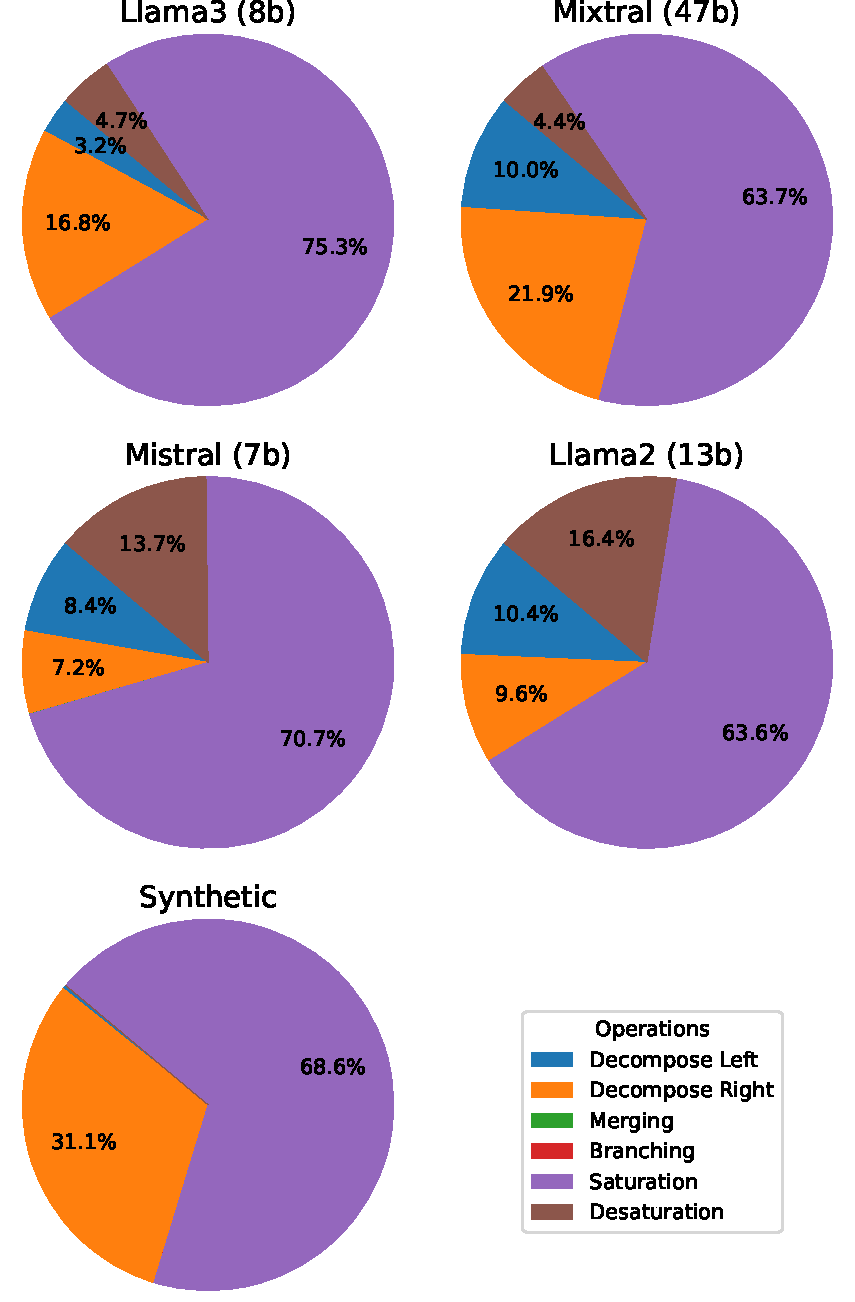
\includegraphics[width=0.75\linewidth]{figures/combined_models}
    \caption[Learner operations by teacher type]{%
        Aggregated results of the operations performed by the learner during the \gls{PAC} learning of all the ontologies grouped by teacher type (\glspl{LLM} and synthetic).
    }
    \label{fig:learner-operations-models}
\end{figure}
%
\begin{figure}
    \centering
    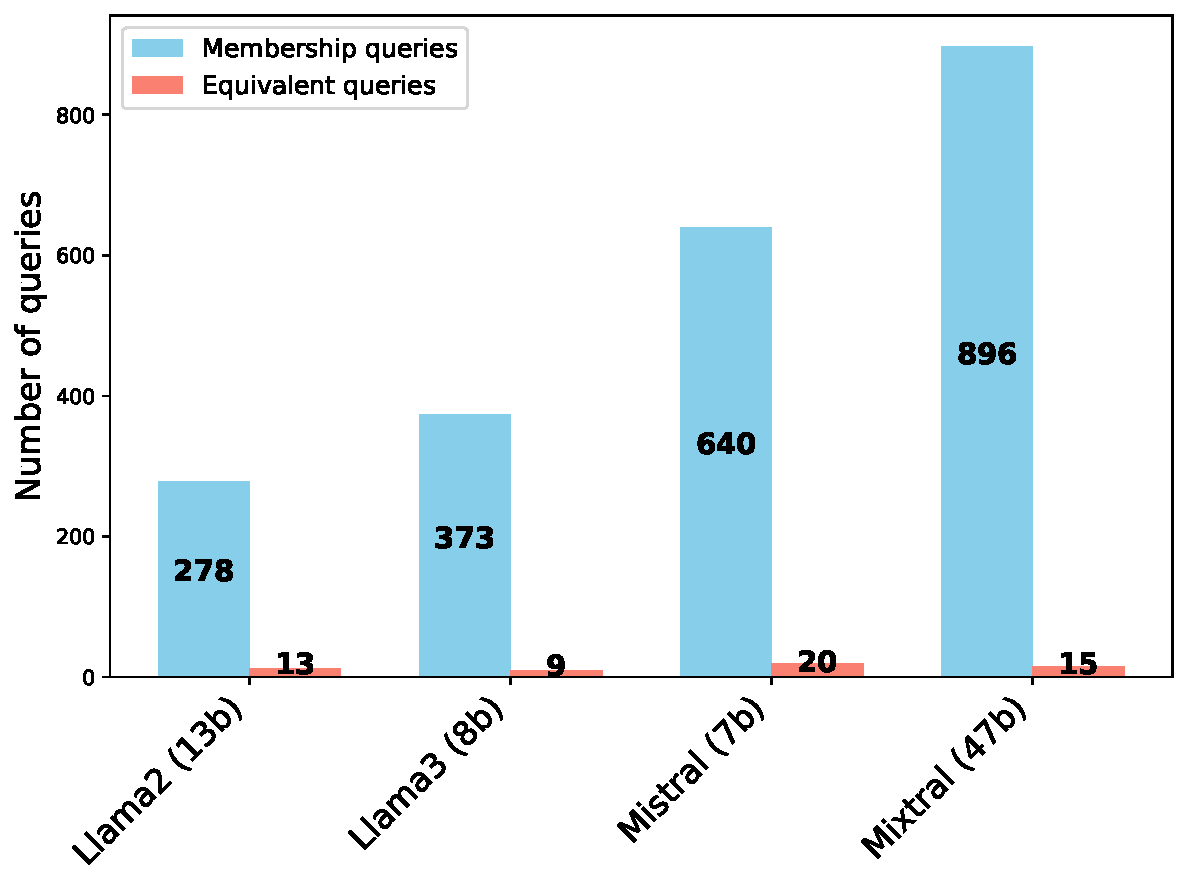
\includegraphics[width=0.75\linewidth]{figures/query_counts_by_model}
    \caption[Queries by \gls{LLM}]{%
        Average number of membership and (simulated) equivalence queries grouped by \gls{LLM}.
        %
        Each equivalence query is simulated by a batch of randomly generated queries.
    }
    \label{fig:queries}
\end{figure}
%
To validate our implementation, we tested ExactLearner+LLM with a synthetic teacher capable of perfectly answering membership queries.
%
\Cref{tab:results-synthetic} reports the results.
%
Precision is always 1, as the synthetic teacher has full knowledge of the target ontology.
%
Other metrics may not reach 1 due to the PAC stopping criterion with \(\epsilon = 0.2\) and \(\delta = 0.1\).

%
\paragraph{Learner Behavior Analysis}
\label{par:learner-behavior-analysis}
%
\Cref{fig:learner-operations-models} illustrates the operations performed by the learner, grouped by teacher type.
%
For \glspl{LLM}, saturation is the most frequent operation, followed by right decomposition, left decomposition, and desaturation.
%
In contrast, the synthetic teacher primarily involves saturation and right decomposition.

%
\Cref{fig:queries} shows the average number of membership and simulated equivalence queries per \gls{LLM}.
%
The choice of \gls{LLM} significantly impacts the number of queries posed during learning.

%
Simplification and splitting operations improved F1-scores across most \gls{LLM} and prompt combinations, confirming \textbf{hypothesis (5)}.
%
For instance, the Mistral model with natural language prompts saw an F1-score increase from approximately 0.5 to 0.7.

%
\subsection{Conclusion and Discussion}
\label{subsec:actively-learning-conclusion}
%
We introduced \emph{ExactLearner+LLM}, an extension of the ExactLearner tool that leverages \glspl{LLM} as teachers to learn \EL ontologies.
%
The tool addresses challenges such as query input format, unexpected responses, and logical consistency.
%
Mechanisms like query simplification and splitting were implemented to adapt to \gls{LLM} behavior.

%
Experimental results demonstrate statistical evidence of correlation between learned and original ontologies.
%
Key findings include:
%
\begin{enumerate}
    \item Concept inclusions of the form \(A \sqsubseteq B\) are easier to learn than \(A \sqsubseteq \exists r.B\) or \(\exists r.B \sqsubseteq A\), leading to worse results for ontologies with more of the latter types.
    %
    \item Operations such as saturation, desaturation, and right decomposition were successfully applied.
    %
    \item The Mistral model outperformed larger models like Mixtral.
    %
    \item Natural language prompts significantly improved performance compared to Manchester OWL syntax.
\end{enumerate}

%
Our approach guarantees the construction of \EL terminologies with a specified vocabulary, even in a zero-shot setting.
%
Future work includes exploring efficient counterexample generation, enhancing ontology language expressivity, and fine-tuning \glspl{LLM} for technical domains like medicine.